\documentclass[11pt,a4paper]{article}
\usepackage[margin=23mm,headheight=14pt,headsep=8.5mm,footskip=10mm]{geometry}
\usepackage{amsmath,amssymb,amsthm}
\usepackage[no-math]{fontspec}
\usepackage{xeCJK}
\setmainfont{Latin Modern Roman}
\setCJKmainfont{FandolSong-Regular.otf}[Script=CustomDefault,Path=assets/fonts/fandol/,BoldFont=FandolSong-Bold.otf,ItalicFont=FandolSong-Regular.otf,BoldItalicFont=FandolSong-Bold.otf]
\setCJKsansfont{FandolSong-Regular.otf}[Script=CustomDefault,Path=assets/fonts/fandol/,BoldFont=FandolSong-Bold.otf]
\xeCJKsetup{PunctStyle=quanjiao,CheckSingle=true}
\usepackage{setspace}
\setstretch{1.12}
\setlength{\parindent}{2em}
\setlength{\parskip}{3pt}
\usepackage{titlesec}
\titleformat{\section}{\centering\normalfont\Large\bfseries}{\thesection.}{0.6em}{}
\titleformat{\subsection}{\normalfont\large\bfseries}{}{0pt}{}
\titlespacing*{\section}{0pt}{1.8\baselineskip}{1.0\baselineskip}
\titlespacing*{\subsection}{0pt}{1.1\baselineskip}{0.5\baselineskip}
\usepackage{enumitem}
\setlist[enumerate]{leftmargin=2em,labelsep=0.5em,itemsep=3pt,parsep=0pt,topsep=6pt}
\providecommand{\tightlist}{\setlength{\itemsep}{3pt}\setlength{\parskip}{0pt}}
\usepackage{needspace}
\newenvironment{statementblock}{\par\Needspace{9\baselineskip}\noindent}{\par\nopagebreak[4]}
\newenvironment{proofblock}{\par\Needspace{4\baselineskip}\noindent}{\par}
\usepackage{fancyhdr}
\pagestyle{fancy}
\fancyhf{}
\fancyhead[L]{\small 数学手记}
\fancyhead[R]{\small 复变函数 · 第二章}
\fancyfoot[C]{\thepage}
\renewcommand{\headrulewidth}{0.4pt}
\usepackage[hidelinks,unicode,bookmarksnumbered=true,linktoc=all]{hyperref}
\usepackage{bookmark}
\bookmarksetup{depth=2}
\hypersetup{pdftitle={复变函数讲义：第二章},pdfauthor={Vincent Arqain},pdfsubject={全纯函数}}
\renewcommand{\contentsname}{目录}
\setcounter{tocdepth}{1}
\setcounter{secnumdepth}{1}
\widowpenalty=10000
\clubpenalty=10000
\displaywidowpenalty=10000
\predisplaypenalty=10000
\interdisplaylinepenalty=10000
\raggedbottom

\usepackage{tabularx,booktabs,array}
\renewcommand{\thesection}{2.\arabic{section}}
\emergencystretch=2em

\usepackage{graphicx}
\usepackage{float}
\floatplacement{figure}{H}
\renewcommand{\figurename}{图}
\makeatletter
\def\maxwidth{\ifdim\Gin@nat@width>\linewidth\linewidth\else\Gin@nat@width\fi}
\def\maxheight{\ifdim\Gin@nat@height>0.72\textheight0.72\textheight\else\Gin@nat@height\fi}
\makeatother
\setkeys{Gin}{width=\maxwidth,height=\maxheight,keepaspectratio}
\providecommand{\pandocbounded}[1]{#1}
\setcounter{tocdepth}{2}
\begin{document}
\begin{center}
{\LARGE\bfseries 复变函数讲义\par}
\vspace{8pt}{\large 第二章\quad 全纯函数\par}
\vspace{6pt}{\small 依史济怀、刘太顺《复变函数》\quad 教材第 27—67 页\par}
\end{center}\vspace{8pt}
本章含5节讲义及全部 74 道习题原题。定义、定理和性质沿用教材的记号与编号；证明补足必要条件、退化情形与关键推导。从复线性微分与 Cauchy--Riemann 方程出发，依次建立保角性、初等函数及其分支、分式线性变换。全纯高阶正则性给出独立补证；各节设可点击定理索引，原题按节跳转。习题不附解答，原题中的疑义另列校勘。
\tableofcontents\clearpage
\section{复变函数的导数}
对应教材 §2.1，第 27---28
页。本章的主线是：复差商要求所有方向给出同一个线性主部；这一限制化为
Cauchy--Riemann
方程，几何上成为旋转与等比伸缩，进而支配初等函数及分式线性变换。

\Needspace{5\baselineskip}
\subsection{定义与线性主部}\label{ch02-s1-ux5b9aux4e49ux4e0eux7ebfux6027ux4e3bux90e8}

\textbf{定义 2.1.1：} 设 \(f:D\to\mathbb C\)，\(D\)
是域，\(z_0\in D\)。若有限极限

\[
f'(z_0)=\lim_{z\to z_0}\frac{f(z)-f(z_0)}{z-z_0}
\qquad\text{(2.1.1)}
\]

存在，称 \(f\) 在 \(z_0\) 处复可微，简称可微。若在 \(D\) 每一点可微，称
\(f\) 在 \(D\) 全纯或解析；若在 \(z_0\) 的某个开邻域全纯，称 \(f\) 在
\(z_0\) 处全纯。教材此处以``解析''作同义词，幂级数刻画到第四章才建立。

极限中的 \(z\) 可以沿任意方式趋近
\(z_0\)。只核对实轴和虚轴两条路径能得到必要条件，不能证明极限存在。

\textbf{等价形式：} \(f\) 在 \(z_0\) 可微，当且仅当存在
\(A\in\mathbb C\)，使

\[
f(z_0+\Delta z)-f(z_0)=A\Delta z+o(|\Delta z|).
\qquad\text{(2.1.2)}
\]

此时 \(A=f'(z_0)\)。

证明：若差商趋于 \(A\)，把差商写成 \(A+\varepsilon(\Delta z)\)，其中
\(\varepsilon\to0\)，相乘即得，且
\(|\varepsilon\Delta z|/|\Delta z|\to0\)。反之，将余项除以
\(\Delta z\ne0\)，其模趋零，故差商趋于
\(A\)。这里的主部是``乘一个复数''，不是任意实线性映射。

\textbf{命题 2.1.2：可微必连续。}

证明：由式（2.1.2），增量的模不超过 \((|A|+o(1))|\Delta z|\)，趋于零。

\textbf{例 2.1.3：} \(f(z)=\bar z\) 处处连续而处处不可微。

证明：\(|\bar z-\bar z_0|=|z-z_0|\) 给出连续性。差商为
\(\overline{\Delta z}/\Delta z\)；沿非零实增量恒为
\(1\)，沿非零纯虚增量恒为 \(-1\)，故极限不存在。相同方法说明
\(\operatorname{Re}z\) 处处不可微。\(|z|\)
在非零点处沿径向与切向的差商极限不同，在零点处 \(|\Delta z|/\Delta z\)
也依方向而变，故处处不可微。

\Needspace{5\baselineskip}
\subsection{单点与邻域}\label{ch02-s1-ux5355ux70b9ux4e0eux90bbux57df}

\textbf{补充辨析：} \(f(z)=|z|^2\) 仅在 \(0\) 可微，且
\(f'(0)=0\)，但在任何点都不全纯。

证明：原点的差商为 \(\bar z\to0\)。在 \(z_0\ne0\)，

\[
\frac{|z_0+h|^2-|z_0|^2}{h}
=\bar z_0+z_0\frac{\bar h}{h}+\bar h.
\]

沿实增量及纯虚增量的极限分别为
\(\bar z_0+z_0\)、\(\bar z_0-z_0\)，二者不同。任一原点邻域都含非零点，所以它虽在原点可微，却不在原点全纯。

``在一点全纯''包含一个邻域的条件；``在一点有复导数''只涉及该点。以后出现的积分表示、高阶可导、局部幂级数均依赖邻域全纯，不能由单点导数推出。

\Needspace{5\baselineskip}
\subsection{导数的运算}\label{ch02-s1-ux5bfcux6570ux7684ux8fd0ux7b97}

\textbf{代数运算法则：} 若 \(f,g\) 在 \(z_0\) 可微，则和、差、积可微；若
\(g(z_0)\ne0\)，商也在 \(z_0\) 可微，且

\[
\begin{aligned}
(f\pm g)'&=f'\pm g',\\
(fg)'&=f'g+fg',\\
(f/g)'&=\frac{f'g-fg'}{g^2}.
\end{aligned}
\]

证明：把 \(\Delta f=f'h+o(|h|)\)、\(\Delta g=g'h+o(|h|)\)
相加、相减即得前式。由

\[
\Delta(fg)=g(z_0)\Delta f+f(z_0)\Delta g+\Delta f\Delta g
\]

及 \(\Delta f\Delta g=O(|h|^2)=o(|h|)\) 得积的公式。连续性保证 \(g\) 在
\(z_0\) 附近不为零；再由

\[
\frac{1/g(z_0+h)-1/g(z_0)}h
=-\frac{g(z_0+h)-g(z_0)}{h\,g(z_0+h)g(z_0)}
\]

得到
\((1/g)'=-g'/g^2\)，与乘积法则合用即得商的公式。在域中逐点应用，便得到相应的全纯性。

\textbf{命题 2.1.4：复合函数的链式法则。} 若
\(f:D_1\to D_2\)、\(g:D_2\to\mathbb C\) 全纯，则 \(h=g\circ f\) 全纯，且

\[
h'(z)=g'(f(z))f'(z).
\]

证明：固定 \(z_0\)，记 \(w_0=f(z_0)\)、\(k=f(z_0+h)-f(z_0)\)。有
\(k=f'(z_0)h+o(|h|)=O(|h|)\)。把 \(g(w_0+k)-g(w_0)\) 写成
\(g'(w_0)k+\eta(k)k\)，规定 \(\eta(0)=0\)，则 \(\eta(k)\to0\)。代入得

\[
g(f(z_0+h))-g(f(z_0))=g'(w_0)f'(z_0)h+o(|h|).
\]

这同时处理了 \(k=0\) 的增量，不需除以可能为零的 \(f(z_0+h)-f(z_0)\)。

\textbf{基本例子：} 常数导数为零，\(z\) 的导数为 \(1\)。由乘积法则归纳得
\((z^n)'=nz^{n-1}\)（\(n\ge1\)）；因此多项式在全平面全纯，有理函数在分母不为零处全纯。

\Needspace{5\baselineskip}
\subsection{定理索引}\label{ch02-s1-ux5b9aux7406ux7d22ux5f15}

本节索引：\hyperref[ch02-s1-ux5b9aux4e49ux4e0eux7ebfux6027ux4e3bux90e8]{定义
2.1.1、命题 2.1.2} · \hyperref[ch02-s1-ux5bfcux6570ux7684ux8fd0ux7b97]{命题
2.1.4}。

定义 2.1.1 给出复可微与全纯；命题 2.1.2 给出连续性；例 2.1.3
区分连续与复可微；命题 2.1.4
给出复合求导。判断可微时先寻找式（2.1.2）的主部；否定可微时才用不同路径产生矛盾。

\section{Cauchy–Riemann 方程}
对应教材 §2.2，第 29---36 页。记
\(z=x+iy\)、\(f=u+iv\)。本节的核心是：实可微给出两个实方向的统一线性近似，Cauchy--Riemann
方程再把它限制为复线性近似。

\Needspace{5\baselineskip}
\subsection{实线性主部}\label{ch02-s2-ux5b9eux7ebfux6027ux4e3bux90e8}

\textbf{定义 2.2.1：} \(f\) 在 \(z_0=x_0+iy_0\) 实可微，指 \(u,v\)
作为二元实函数在 \((x_0,y_0)\) 可微，即各有全微分余项
\(o(\sqrt{(\Delta x)^2+(\Delta y)^2})\)。合并为

\[
\Delta f=f_x(z_0)\Delta x+f_y(z_0)\Delta y+o(|\Delta z|).
\]

定义教材的微分算子

\[
\frac\partial{\partial z}=\frac12\left(\frac\partial{\partial x}-i\frac\partial{\partial y}\right),\qquad
\frac\partial{\partial\bar z}=\frac12\left(\frac\partial{\partial x}+i\frac\partial{\partial y}\right).
\qquad\text{(2.2.3)}
\]

\textbf{命题 2.2.2：} 实可微等价于

\[
\Delta f=f_z(z_0)\Delta z+f_{\bar z}(z_0)\overline{\Delta z}+o(|\Delta z|).
\qquad\text{(2.2.4)}
\]

证明：把
\(\Delta x=(\Delta z+\overline{\Delta z})/2\)、\(\Delta y=(\Delta z-\overline{\Delta z})/(2i)\)
代入全微分，即得正向；反向代入 \(\Delta z=\Delta x+i\Delta y\)
并取实、虚部即得。系数唯一，因为 \(Ah+B\bar h=0\) 对所有 \(h\)
成立时，取 \(h=1,i\) 分别给出 \(A+B=0\)、\(A-B=0\)。

于是任一实线性映射恰有 \(h\mapsto Ah+B\bar h\) 的形式。将 \(z,\bar z\)
``看作独立变量''是上述算子恒等式的计算规则，不是声称平面上二者能独立取值。直接代入得
\(z_z=1\)、\(z_{\bar z}=0\)、\(\bar z_z=0\)、\(\bar z_{\bar z}=1\)；乘积法则由实偏导的乘积法则得到。

\Needspace{5\baselineskip}
\subsection{复可微的充要条件}\label{ch02-s2-ux590dux53efux5faeux7684ux5145ux8981ux6761ux4ef6}

\textbf{定理 2.2.3：} \(f\) 在 \(z_0\) 复可微，当且仅当它在 \(z_0\)
实可微且 \(f_{\bar z}(z_0)=0\)。此时 \(f'(z_0)=f_z(z_0)\)。

证明：复可微的增量式已经是一个实线性近似；同命题 2.2.2
比较并用系数唯一性，得
\(f_z=f'\)、\(f_{\bar z}=0\)。反之，式（2.2.4）的共轭项为零后，正是复可微的增量式。

计算

\[
f_{\bar z}=\tfrac12(u_x-v_y)+\tfrac i2(v_x+u_y),
\]

便得到 \textbf{定理 2.2.4：} \(f=u+iv\) 在 \(z_0\) 复可微，当且仅当
\(u,v\) 在 \((x_0,y_0)\) 实可微，并满足

\[
u_x=v_y,\qquad u_y=-v_x.
\qquad\text{(2.2.5)}
\]

证明：实部和虚部同时为零等价于 \(f_{\bar z}=0\)，应用定理 2.2.3
即得。代回 \(f_z\) 可得教材的四种导数表示

\[
f'=u_x+iv_x=v_y+iv_x=u_x-iu_y=v_y-iu_y.
\]

在域 \(D\) 逐点应用该判据即可判定全纯。它不是只在某一点核对一次方程。

\Needspace{5\baselineskip}
\subsection{正则性不能遗漏}\label{ch02-s2-ux6b63ux5219ux6027ux4e0dux80fdux9057ux6f0f}

记 \(C(D)\) 为连续函数类，\(C^k(D)\) 为有 \(k\)
阶连续实偏导的函数类，\(H(D)\) 为全纯函数类。\(C^1\)
是保证实可微的常用充分条件，但单点复可微的判据本身不要求偏导在邻域连续。

\textbf{\(C^1\) 充分条件的证明：} 对实函数
\(u\)，把增量沿坐标方向拆成两段，实一元中值定理给出

\[
\Delta u=u_x(\xi,y_0+\Delta y)\Delta x+u_y(x_0,\eta)\Delta y.
\]

偏导在 \((x_0,y_0)\) 连续，使两系数分别等于
\(u_x(x_0,y_0)+o(1)\)、\(u_y(x_0,y_0)+o(1)\)。由
\(|\Delta x|+|\Delta y|\le\sqrt2|\Delta z|\) 得全微分余项；\(v\)
同理。所以 \(f\in C^1(D)\) 且处处满足（2.2.5）必全纯。

\textbf{仅有偏导和方程仍不够。} 例如令

\[
f(x+iy)=\begin{cases}\dfrac{x^3}{x^2+y^2}+i\dfrac{y^3}{x^2+y^2},&(x,y)\ne(0,0),\\0,&(x,y)=(0,0).\end{cases}
\]

原点处 \(u_x=v_y=1\)、\(u_y=v_x=0\)，满足方程；沿实轴差商为 \(1\)，沿
\(y=x\) 差商为
\(1/2\)，故不复可微。缺失的是实可微，而不是方程的代数形式。

\textbf{例 2.2.5、2.2.6：} \(z^n\) 实可微且
\((z^n)_{\bar z}=0\)，故全纯，导数为
\(nz^{n-1}\)；\(e^{|z|^2}=e^{z\bar z}\) 属于 \(C^\infty(\mathbb C)\)，而

\[
(e^{z\bar z})_{\bar z}=ze^{z\bar z}.
\]

它仅在零点复可微，并在任何点都不全纯。无穷阶实光滑不能替代复线性条件。

对 \(k>1\)，有

\[
H(D)\subset C^\infty(D)\subset C^k(D)\subset C^1(D)\subset C(D).
\]

其中第一个包含关系不是 Cauchy--Riemann 方程直接给出的；教材预引定理
3.4.4。本节末尾给出独立补证，随后使用二阶偏导、实逆函数定理时便不会隐含未经证明的正则性。

\Needspace{5\baselineskip}
\subsection{调和与共轭调和}\label{ch02-s2-ux8c03ux548cux4e0eux5171ux8f6dux8c03ux548c}

\textbf{定义 2.2.7：} 实值函数 \(u\in C^2(D)\) 满足

\[
\Delta u=u_{xx}+u_{yy}=0
\]

时称为调和函数，\(\Delta=\partial_x^2+\partial_y^2\) 是 Laplace 算子。

\textbf{命题 2.2.8：} 对 \(u\in C^2(D)\)，

\[
\Delta u=4\frac{\partial^2u}{\partial z\partial\bar z}.
\]

证明：将 \((\partial_x-i\partial_y)(\partial_x+i\partial_y)\)
展开，混合项为 \(i(u_{xy}-u_{yx})=0\)，余下 \(u_{xx}+u_{yy}\)。交换
\(z,\bar z\) 次序也一样；\(C^2\) 正是交换混合偏导的依据。

\textbf{定理 2.2.9：} 若 \(f=u+iv\in H(D)\)，则 \(u,v\) 均调和。

证明：由本节末尾的正则性补证，\(u,v\in C^2(D)\)。对
\(u_x=v_y\)、\(u_y=-v_x\) 分别求导，得

\[
u_{xx}+u_{yy}=v_{yx}-v_{xy}=0,\qquad
v_{xx}+v_{yy}=-u_{yx}+u_{xy}=0.
\]

\textbf{定义 2.2.10：} 若调和函数 \(u,v\) 满足（2.2.5），称 \(v\) 为
\(u\) 的共轭调和函数。次序有方向性：\(v\) 是 \(u\) 的共轭时，\(-u\) 是
\(v\) 的共轭。

\textbf{定理 2.2.11：} 单连通域 \(D\) 上的调和函数 \(u\)
存在共轭调和函数 \(v\)，使 \(u+iv\in H(D)\)。

证明：希望得到 \(v_x=-u_y\)、\(v_y=u_x\)，自然构造实微分形式

\[
\omega=-u_y\,dx+u_x\,dy.
\]

因 \(u\in C^2\) 且 \((u_x)_x=(-u_y)_y\)，\(\omega\)
闭合。在小矩形上，Green
公式给出闭路积分为零，从而存在局部势函数。单连通域内闭路可缩为一点：将收缩同伦的参数方形分成足够细的网格，使每个小格的像落在一个局部势函数邻域内；沿各小格边的势差相加为零，内边两两抵消，外边只剩原闭路与常值路径。故原闭路的积分为零。这里对连续同伦的边用邻域内分段光滑路径替代，局部势差保证替代不改变结果。这就是实微积分中闭合形式在单连通域上有势函数的理由。

固定 \((x_0,y_0)\in D\)，定义

\[
v(x,y)=\int_{(x_0,y_0)}^{(x,y)}(-u_y\,dx+u_x\,dy).
\]

积分与分段光滑路径无关。在终点加一小段水平或竖直线段，直接得到
\(v_x=-u_y\)、\(v_y=u_x\)，二者为 \(C^1\)，故 \(v\in C^2\)。又
\(v_{xx}+v_{yy}=-u_{yx}+u_{xy}=0\)，且满足（2.2.5），所以 \(u+iv\)
全纯。

若 \(v_1,v_2\) 都是 \(u\) 的共轭，则 \(v_1-v_2\)
的梯度为零，沿域内折线积分得其为常数。单连通是存在性的充分条件；一般域上的准确障碍是
\(\omega\)
的闭路积分是否全为零。此构造把``寻找虚部''变成``检验微分形式是否具有单值势函数''。

\Needspace{5\baselineskip}
\subsection{全纯正则性的补证}\label{ch02-s2-ux5168ux7eafux6b63ux5219ux6027ux7684ux8865ux8bc1}

本段仅用复可微的定义、实曲线积分与紧性，补足教材预引的
\(H(D)\subset C^\infty(D)\)；并不以调和性、导数连续或幂级数展开为前提。

\textbf{局部积分引理：} 若 \(f\) 在闭三角形及其邻域全纯，则
\(\int_{\partial T}f(\zeta)\,d\zeta=0\)。此处分段光滑曲线积分按实积分定义为
\(\int f(\gamma(t))\gamma'(t)\,dt\)。

证明：连接三边中点，把 \(T\)
分为四个小三角形。内边相消，至少有一个子三角形 \(T_1\)
的边界积分模不小于原值的 \(1/4\)。重复选取，得到套闭三角形
\(T_n\)，直径、周长分别缩为 \(2^{-n}d\)、\(2^{-n}\ell\)，公共点为
\(a\)，且 \(|I(T)|\le4^n|I(T_n)|\)。在 \(a\) 处写

\[
f(\zeta)=f(a)+f'(a)(\zeta-a)+r(\zeta),\qquad
|r(\zeta)|\le\varepsilon|\zeta-a|
\]

（\(n\) 充分大）。常数及一次项沿闭路积分为零，因为分别有显式原函数
\(f(a)\zeta\) 和 \(f'(a)(\zeta-a)^2/2\)。因此

\[
|I(T)|\le4^n\varepsilon(2^{-n}d)(2^{-n}\ell)=\varepsilon d\ell.
\]

令 \(\varepsilon\downarrow0\)，引理得证。这是三角形形式的 Goursat 论证。

取闭正方形 \(Q\subset D\)，\(z\) 在其内部。以 \(z\) 为中心挖去边长
\(2\varepsilon\) 的小正方形 \(Q_\varepsilon\)。在其间的多边形区域上对
\(f(\zeta)/(\zeta-z)\)
使用引理：有限三角剖分后内边相消，故两条正向边界积分相等。由连续性，

\[
\left|\int_{\partial Q_\varepsilon}\frac{f(\zeta)-f(z)}{\zeta-z}\,d\zeta\right|
\le8\sup_{\partial Q_\varepsilon}|f(\zeta)-f(z)|\longrightarrow0.
\]

直接参数计算小正方形上的积分
\(\int d\zeta/(\zeta-z)=2\pi i\)：每边的实部是 \(\log|\zeta-z|\)
的增量，总和为零；连续辐角每边增加 \(\pi/2\)，虚部总和为 \(2\pi\)。于是

\[
f(z)=\frac1{2\pi i}\int_{\partial Q}\frac{f(\zeta)}{\zeta-z}\,d\zeta.
\qquad\text{(补2.2-A)}
\]

在 \(Q\) 内任一紧子方形上，\(|\zeta-z|\) 有统一正下界。核函数对 \(z\)
的各阶差商一致收敛到相应导数，可在有限长度边界上逐次交换求导与积分，得

\[
f^{(n)}(z)=\frac{n!}{2\pi i}\int_{\partial Q}\frac{f(\zeta)}{(\zeta-z)^{n+1}}\,d\zeta,\qquad n\ge0.
\]

各积分连续；或者直接对核作任意阶 \(x,y\) 偏导，得到全部连续实偏导。因此
\(f\in C^\infty(D)\)。每一点均可放入这样的正方形，故结论覆盖整个域。第三章会系统发展这一积分表示。

\Needspace{5\baselineskip}
\subsection{定理索引}\label{ch02-s2-ux5b9aux7406ux7d22ux5f15}

本节索引：\hyperref[ch02-s2-ux5b9eux7ebfux6027ux4e3bux90e8]{定义 2.2.1、命题
2.2.2} ·
\hyperref[ch02-s2-ux590dux53efux5faeux7684ux5145ux8981ux6761ux4ef6]{定理
2.2.3---2.2.4} ·
\hyperref[ch02-s2-ux8c03ux548cux4e0eux5171ux8f6dux8c03ux548c]{编号
2.2.7---2.2.11 的定义、命题与定理} ·
\hyperref[ch02-s2-ux5168ux7eafux6b63ux5219ux6027ux7684ux8865ux8bc1]{正则性补证}。

定义 2.2.1、命题 2.2.2 对应实可微与实线性主部；定理 2.2.3---2.2.4
对应复可微判据；定义 2.2.7、命题 2.2.8 对应调和与 Laplace 分解；定理
2.2.9、定义 2.2.10、定理 2.2.11
对应全纯函数与共轭调和函数。补充积分引理独立证明正则性，不占用教材编号。

\section{导数的几何意义}
对应教材 §2.3，第 36---39 页。设 \(f\) 在 \(z_0\)
附近全纯，\(w_0=f(z_0)\)。真正控制局部图形的是
\(\Delta w=f'(z_0)\Delta z+o(|\Delta z|)\)，而不是函数式表面是否复杂。

\Needspace{5\baselineskip}
\subsection{转动角}\label{ch02-s3-ux8f6cux52a8ux89d2}

过 \(z_0\) 的有向光滑曲线记为
\(z=\gamma(t)\)，\(\gamma(a)=z_0\)、\(\gamma'(a)\ne0\)。像曲线为
\(w=\sigma(t)=f(\gamma(t))\)。由实参数链式法则，

\[
\sigma'(a)=f'(z_0)\gamma'(a).
\]

证明也可以直接完成：\(\gamma(a+h)-\gamma(a)=\gamma'(a)h+o(|h|)\)，代入
\(f\) 的增量式，再除以实数 \(h\) 取极限即可。

若 \(f'(z_0)\ne0\)，像曲线切向量非零，因而

\[
\operatorname{Arg}\sigma'(a)-\operatorname{Arg}\gamma'(a)
=\operatorname{Arg}f'(z_0)\pmod{2\pi}.
\qquad\text{(2.3.1)}
\]

这就是转动角，与所取曲线无关。这里是辐角同余；不能把主辐角相减后得到的实数不经调整就认作唯一的转动角。

\Needspace{5\baselineskip}
\subsection{保角定理}\label{ch02-s3-ux4fddux89d2ux5b9aux7406}

\textbf{定理 2.3.1：}
全纯函数在导数非零的点处保角，即保持任意两条正则曲线的有向夹角。

证明：取两条曲线 \(\gamma_1,\gamma_2\) 及其像
\(\sigma_1,\sigma_2\)。将式（2.3.1）相减，公共的转动角消去，得到

\[
\operatorname{Arg}\sigma_2'(a)-\operatorname{Arg}\sigma_1'(a)
=\operatorname{Arg}\gamma_2'(a)-\operatorname{Arg}\gamma_1'(a)\pmod{2\pi}.
\qquad\text{(2.3.2)}
\]

所以不仅夹角大小相同，旋转方向也保持。关键构造是对两条切向量乘上同一个非零复数；若分别伸缩两个坐标方向，夹角一般不会保持。

等价地，写 \(f'(z_0)=\alpha+i\beta=re^{i\theta}\)，实微分矩阵为

\[
Df(z_0)=\begin{pmatrix}\alpha&-\beta\\\beta&\alpha\end{pmatrix}
=r\begin{pmatrix}\cos\theta&-\sin\theta\\\sin\theta&\cos\theta\end{pmatrix}.
\]

证明：将 \((\alpha+i\beta)(\Delta x+i\Delta y)\)
分离实、虚部，即得矩阵；再用
\(\alpha=r\cos\theta\)、\(\beta=r\sin\theta\) 得分解。于是
\(Df^{\mathsf T}Df=r^2I\)、\(\det Df=r^2>0\)，分别表达各方向伸缩相同与定向保持。

\Needspace{5\baselineskip}
\subsection{伸缩率与局部共形}\label{ch02-s3-ux4f38ux7f29ux7387ux4e0eux5c40ux90e8ux5171ux5f62}

\textbf{伸缩率：} 不论趋近路径如何，

\[
\lim_{z\to z_0}\frac{|f(z)-f(z_0)|}{|z-z_0|}=|f'(z_0)|.
\]

证明：复差商趋于 \(f'(z_0)\)，再取连续的模函数即可。对正则曲线，也有
\(|\sigma'(a)|/|\gamma'(a)|=|f'(z_0)|\)。

因此当 \(f'(z_0)\ne0\) 时，微分把以 \(z_0\)
为顶点的小三角形变为同向相似的三角形。实际像是曲边三角形，``相似''准确地说是尺度趋零时的一阶结论。教材称这样的映射为共形映射。

\textbf{局部单叶与逆映射：} 若 \(f\) 在 \(z_0\) 邻域全纯且
\(f'(z_0)\ne0\)，则存在邻域 \(U,V\)，使 \(f:U\to V\) 一一对应，其逆
\(g\) 全纯，且

\[
g'(f(z))=\frac1{f'(z)}.
\]

证明：§2.2 已证 \(f\in C^1\)，而
\(\det Df(z_0)=|f'(z_0)|^2>0\)。实逆函数定理给出 \(C^1\) 局部逆；缩小
\(U\) 后 \(f'\) 始终非零。逆矩阵对应乘以
\(1/f'(z)\)，故逆的实微分复线性，由定理 2.2.3
得其全纯和上述导数公式。这里所用实逆函数定理是多元微积分的前置工具。

\Needspace{5\baselineskip}
\subsection{条件与反例}\label{ch02-s3-ux6761ux4ef6ux4e0eux53cdux4f8b}

\textbf{零导数不可直接套用保角结论。} \(f(z)=z^2\)
在原点导数为零。两条射线
\(te^{i\theta_1}\)、\(te^{i\theta_2}\)（\(t\ge0\)）的像分别在辐角
\(2\theta_1,2\theta_2\) 的射线上；例如夹角 \(\pi/4\) 变为
\(\pi/2\)。原参数下两条像曲线在零点速度均为零，定理证明中的切向量辐角无定义。由此可见非零条件不是装饰。

\textbf{局部与整体不同。} \(z^2\) 在 \(\mathbb C\setminus\{0\}\)
的导数处处非零，因此处处局部共形；但 \(z\) 与 \(-z\)
的像相同，故并非全局单叶。全局单叶还需要控制不同点是否发生重合。

\textbf{保角与反保角不同。} 共轭映射 \(z\mapsto\bar z\)
保持夹角的绝对大小，却把有向角变为相反数；其实微分行列式为
\(-1\)，且处处不复可微。教材的保角要求旋转方向也保持，因此不包含这一情形。

对一道映射题，应先明确作用域与单叶性，再检查导数非零；确定边界像之后，还须用内部点或符号判断像域究竟位于边界哪一侧。

\Needspace{5\baselineskip}
\subsection{定理索引}\label{ch02-s3-ux5b9aux7406ux7d22ux5f15}

本节索引：\hyperref[ch02-s3-ux8f6cux52a8ux89d2]{转动角} ·
\hyperref[ch02-s3-ux4fddux89d2ux5b9aux7406]{定理 2.3.1} ·
\hyperref[ch02-s3-ux4f38ux7f29ux7387ux4e0eux5c40ux90e8ux5171ux5f62]{伸缩率与局部逆}。

式（2.3.1）刻画转动角，定理 2.3.1
与式（2.3.2）刻画保角性；模差商给出伸缩率。局部逆的论证使用 §2.2
已补证的正则性和实逆函数定理，不预设``复可微自动具有连续导数''。

\section{初等全纯函数}
对应教材 §2.4，第 39---53 页。沿用教材：\(\operatorname{Arg}z\)
表示多值辐角，\(\arg z\) 表示选定主值；\(\operatorname{Log}z\)
表示多值对数，\(\log z\)
表示主支。必须同时记录函数式、定义域、割线和分支归一化。

\Needspace{5\baselineskip}
\subsection{指数函数}\label{ch02-s4-ux6307ux6570ux51fdux6570}

对 \(z=x+iy\)，定义

\[
e^z=e^x(\cos y+i\sin y).
\]

这个定义只使用实指数及实三角函数，无须预先使用复幂级数。它在实轴上还原实指数，在虚轴上给出
Euler 公式 \(e^{iy}=\cos y+i\sin y\)。

\textbf{教材性质（1）---（5）：} \(e^z\)
在全平面全纯，\((e^z)'=e^z\)；\(|e^z|=e^{\operatorname{Re}z}>0\)；\(e^{z_1+z_2}=e^{z_1}e^{z_2}\)；它以
\(2\pi i\) 为周期，且所有周期恰为 \(2k\pi i\)。

证明：实部 \(u=e^x\cos y\)、虚部 \(v=e^x\sin y\) 为 \(C^\infty\)，且
\(u_x=v_y\)、\(u_y=-v_x\)，于是全纯，\(u_x+iv_x=e^z\)
给出导数。平方取模得
\(|e^z|^2=e^{2x}\)，故不取零值。用实三角加法公式相乘得指数相加法则。若
\(e^{z_1}=e^{z_2}\)，比较模得 \(x_1=x_2\)，再比较单位圆上的点得
\(y_1-y_2\in2\pi\mathbb Z\)。因此

\[
e^{z_1}=e^{z_2}\iff z_1-z_2\in2\pi i\mathbb Z,
\]

也同时证明了周期的全部可能取值。

\textbf{定义 2.4.1：} 在域 \(D\) 上一一的函数称为单叶函数，\(D\)
称为单叶性域。

\textbf{映射性质：} \(e^z\) 将带状域
\(\alpha<\operatorname{Im}z<\alpha+2\pi\) 单叶地映到去掉射线
\(\{re^{i\alpha}:r\ge0\}\) 的平面；较窄带状域映到相应角域。

证明：两点虚部差绝对值小于
\(2\pi\)，故上面的等价式给出单射。对射线外每个 \(w\)，唯一选取
\(\theta\in(\alpha,\alpha+2\pi)\) 使 \(w=|w|e^{i\theta}\)，令
\(z=\log|w|+i\theta\)
即得满射。水平直线映为射线，竖直直线映为圆周，因为分别固定辐角和模。教材第
41 页``除去正实轴''在这里包含除去原点，指数永不取零。

\Needspace{5\baselineskip}
\subsection{对数函数}\label{ch02-s4-ux5bf9ux6570ux51fdux6570}

对 \(z\ne0\)，由 \(e^w=z\) 解得全部值

\[
\operatorname{Log}z=\log|z|+i\arg z+2k\pi i,\qquad k\in\mathbb Z.
\]

证明：写 \(w=u+iv\)，由模得 \(e^u=|z|\)，由辐角得
\(v=\arg z+2k\pi\)；反向代入可验证全部是解。\(z=0\) 没有对数。

\textbf{定理 2.4.2：} 若 \(D\subset\mathbb C\setminus\{0\}\)
单连通，则存在无穷多个单值全纯函数 \(\varphi_k\)，满足

\[
e^{\varphi_k(z)}=z,\qquad \varphi_k'(z)=\frac1z.
\]

它们恰相差常数 \(2k\pi i\)。

证明：令 \(u=\log|z|=\tfrac12\log(x^2+y^2)\)。直接计算

\[
u_x=\frac{x}{x^2+y^2},\quad u_y=\frac{y}{x^2+y^2},\quad
u_{xx}+u_{yy}=0.
\]

由定理 2.2.11，存在共轭调和函数 \(v\)，故 \(F=u+iv\) 全纯，并且

\[
F'=u_x-iu_y=\frac1z.
\]

于是 \((e^F/z)'=0\)。域上导数恒零的函数为常数：由 Cauchy--Riemann
方程，其两个实分量的梯度为零，沿折线应用一元中值定理即可。因此
\(e^F/z=c\)。又 \(|c|=e^u/|z|=1\)，取实数 \(\theta\) 使
\(c=e^{i\theta}\)，令 \(\varphi_0=F-i\theta\)，即有
\(e^{\varphi_0}=z\)。加 \(2k\pi i\) 得全部分支。若 \(\psi\)
是另一分支，则连续函数 \(\psi-\varphi_0\) 取值于离散集
\(2\pi i\mathbb Z\)；域连通，故它恒等于其中一个值。

这一证明先构造连续辐角，而不是直接把主辐角加固定
\(2k\pi\)。后者在跨过负实轴的单连通域上未必连续；教材第 42
页的简写须作此补足。

\textbf{主支与映射：} 在 \(D_0=\mathbb C\setminus(-\infty,0]\)，取
\(-\pi<\arg z<\pi\)，定义 \(\log z=\log|z|+i\arg z\)。它是指数在
\(-\pi<\operatorname{Im}w<\pi\) 上的逆。

证明：指数在此带状域单叶且导数不为零，§2.3
的局部逆与上述全局一一对应相容，故逆全纯，导数为
\(1/z\)。其他分支给出竖直平移 \(2k\pi i\) 后的带状域。一般割去辐角为
\(\alpha\) 的射线时，应取
\(\alpha<\arg z<\alpha+2\pi\)，这时得到的是该割线对应的分支。

\textbf{定义 2.4.3：}
沿某点周围充分小的闭曲线连续延拓后，函数值变到另一分支，则该点是支点。绕
\(0\) 一周，连续辐角增 \(2\pi\)，对数增 \(2\pi i\)，故 \(0\)
是支点。令局部坐标 \(\zeta=1/z\)，则对数变为
\(-\operatorname{Log}\zeta\)，故 \(\infty\)
也是支点。割线是为选取分支而人为去掉的路径，路径上的一般点并非支点。

\textbf{分支运算的限制：}
在各式有定义处，\(\log(zw)-\log z-\log w\in2\pi i\mathbb Z\)，但未必为零。

证明：两边指数相同，用指数的周期判据即可。例如
\(z=w=e^{3\pi i/4}\)，左边两项主对数之和为
\(3\pi i/2\)，而乘积的主对数为
\(-\pi i/2\)。多值集合间的等式与固定分支间的等式必须分开判断。

\Needspace{5\baselineskip}
\subsection{幂函数}\label{ch02-s4-ux5e42ux51fdux6570}

\textbf{定义 2.4.4：}
全平面全纯的函数称为整函数。\(z^n\)（\(n\ge1\)）为整函数，导数
\(nz^{n-1}\)。当 \(n\ge2\)，它除原点外局部保角；\(n=1\) 在原点也保角。

\textbf{幂映射的单叶性：} 对 \(z_j=r_je^{i\theta_j}\ne0\)，

\[
z_1^n=z_2^n\iff r_1=r_2,\quad\theta_1-\theta_2\in\frac{2\pi}{n}\mathbb Z.
\]

证明：先比较模，再比较单位圆上的角度。故开角域
\(\alpha<\arg z<\beta\)、\(0<\beta-\alpha\le2\pi/n\)
是单叶性域，像为辐角在 \(n\alpha,n\beta\)
间的角域（辐角在所取连续区间内理解）。它将射线的角度乘以
\(n\)，将半径变为 \(r^n\)；\(z^2\) 因此把第一象限映为上半平面。

\textbf{开方：} 在去掉正实轴及原点的平面上选 \(0<\theta<2\pi\)，则
\(z^{1/n}\) 的 \(n\) 个分支为

\[
\varphi_k(z)=|z|^{1/n}\exp\!\left(i\frac{\theta+2k\pi}{n}\right),\qquad 0\le k<n.
\]

证明：以该域上的对数分支 \(L\) 写为
\(\exp((L+2k\pi i)/n)\)，故全纯，\(n\) 次方为 \(z\)，彼此的比为不同的
\(n\) 次单位根，因而恰有 \(n\) 支。\(k=0\) 的分支把此割线平面单叶地映为
\(0<\arg w<2\pi/n\)，为教材在这个割线约定下的``主支''；它与负实轴割线的通常主值约定不同，使用时必须说明。

\textbf{一般复幂：} 设 \(\mu=a+bi\)，定义多值函数
\(z^\mu=e^{\mu\operatorname{Log}z}\)。在固定对数分支 \(L\) 上定义
\(w_k=e^{\mu(L+2k\pi i)}\)，则

\[
\begin{aligned}
w_k(z)&=e^{a\log|z|-b(\theta+2k\pi)}
 e^{i[b\log|z|+a(\theta+2k\pi)]},\\
\frac{w_{k+1}(z)}{w_k(z)}&=e^{2\pi i\mu},\\
w_k'(z)&=\frac{\mu}{z}w_k(z)=\mu e^{(\mu-1)(L(z)+2k\pi i)}.
\end{aligned}
\]

证明：展开 \((a+bi)(\log|z|+i\theta+2k\pi i)\) 得第一式，比较相邻 \(k\)
得第二式，链式法则及 \(L'=1/z\) 得第三式。导数中 \(z^{\mu-1}\)
必须沿用同一个对数分支。

当 \(\mu\in\mathbb Z\) 时只有一个值；当 \(\mu=p/q\)
为既约有理数、\(q>0\) 时恰有 \(q\) 个值；当 \(\mu\) 为实无理数或
\(\operatorname{Im}\mu\ne0\) 时有无穷多个值。

证明：两支相同当且仅当 \(e^{2\pi i(k-l)\mu}=1\)。若 \(b\ne0\)，取模即得
\(k=l\)；若 \(b=0\)，条件为
\((k-l)a\in\mathbb Z\)，分别给出以上三种情形。非整数幂在 \(0,\infty\)
有分支现象；整数负幂虽在零点有极点，却不是支点。

\Needspace{5\baselineskip}
\subsection{割缝域的映射构造}\label{ch02-s4-ux5272ux7f1dux57dfux7684ux6620ux5c04ux6784ux9020}

\textbf{例 2.4.5：} 上半平面去掉竖直割缝
\(\{a+iy:0<y\le h\}\)（\(a\in\mathbb R,h>0\)）后，可取

\[
w=\sqrt{(z-a)^2+h^2},
\]

其中平方根取 \(0<\operatorname{Arg}((z-a)^2+h^2)<2\pi\) 对应的一支，使
\(\operatorname{Im}w>0\)。

证明与构造：先平移 \(\zeta=z-a\)，把割缝移到虚轴；\(\zeta^2\)
将上半平面一一映到 \(\mathbb C\setminus[0,\infty)\)，并把被删割缝映到
\([-h^2,0)\)，所以删缝后的像为 \(\mathbb C\setminus[-h^2,\infty)\)。加
\(h^2\)
后成为正实轴割线平面，再开平方映为上半平面。每一步均单叶全纯，故复合也是。教材原式
\(0<y<h\) 未删顶点，会使所称``域''不开放；作为割缝域须连同顶点删去。

\textbf{例 2.4.6：} 带状域 \(0<\operatorname{Im}z<2\) 去掉割缝
\(\{x+i:x\le-1\}\) 后，可取

\[
w=\sqrt{e^{\pi z}+e^{-\pi}},\qquad \operatorname{Im}w>0.
\]

证明与构造：\(\zeta=e^{\pi z/2}\) 把带状域单叶地映到上半平面，把割缝映到
\(\{it:0<t\le e^{-\pi/2}\}\)。再用例
2.4.5，便得上述公式。这里也把割缝端点包含在删除集合中。

两例的自然想法相同：先把复杂边界变成射线或线段，再让幂函数展开角度，最后用已确定的逆分支恢复目标半平面。只给根号公式而不说明其值域，尚未确定一个映射。

\Needspace{5\baselineskip}
\subsection{三角函数}\label{ch02-s4-ux4e09ux89d2ux51fdux6570}

定义

\[
\cos z=\frac{e^{iz}+e^{-iz}}2,\qquad
\sin z=\frac{e^{iz}-e^{-iz}}{2i}.
\]

\textbf{教材性质（1）---（7）：}
它们为整函数，\((\cos z)'=-\sin z\)、\((\sin z)'=\cos z\)，均以 \(2\pi\)
为周期；余弦偶、正弦奇；加法公式成立；\(\cos^2z+\sin^2z=1\)、\(\sin2z=2\sin z\cos z\)；正弦的零点恰为
\(k\pi\)，余弦的零点恰为 \(\pi/2+k\pi\)；两者在复平面均无界。

证明：全纯性与导数由指数和链式法则得到。将 \(z\) 换为
\(z+2\pi\)，两个指数不变，给出周期；换成
\(-z\)，两个指数互换，给出奇偶性。令 \(A=e^{iz}\)、\(B=e^{iw}\)，例如

\[
\begin{aligned}
\cos z\cos w-\sin z\sin w
&=\tfrac14[(A+A^{-1})(B+B^{-1})+(A-A^{-1})(B-B^{-1})]\\
&=\tfrac12(AB+(AB)^{-1})=\cos(z+w).
\end{aligned}
\]

同样将 \((A-A^{-1})(B+B^{-1})+(A+A^{-1})(B-B^{-1})\) 展开，得
\(2(AB-(AB)^{-1})\)，除以 \(4i\) 即得正弦加法公式。分别令
\(w=-z\)、\(w=z\)，得到平方和与倍角公式。

\(\sin z=0\) 等价于 \(e^{2iz}=1\)，故 \(z=k\pi\)；\(\cos z=0\) 等价于
\(e^{2iz}=-1\)，故 \(z=\pi/2+k\pi\)，其中
\(k\in\mathbb Z\)。最后，\(\cos(iy)=(e^y+e^{-y})/2\to\infty\)，\(\sin(\pi/2+iy)=\cos(iy)\)，证明两者无界。

定义
\(\tan z=\sin z/\cos z\)、\(\cot z=\cos z/\sin z\)。由商法则，它们分别在排除上述分母零点的域全纯，导数为
\(1/\cos^2z\)、\(-1/\sin^2z\)。因此实三角函数的代数恒等式继续成立，实轴上的有界性却不能推广到复平面。

\Needspace{5\baselineskip}
\subsection{代数多值函数}\label{ch02-s4-ux4ee3ux6570ux591aux503cux51fdux6570}

考虑教材 §2.4.5 的函数

\[
w=\sqrt[n]{(z-a_1)^{\beta_1}\cdots(z-a_m)^{\beta_m}},
\]

其中 \(a_j\) 互异，\(\beta_j\in\mathbb Z\)，\(n\ge1\)。相同的 \(a_j\)
应先合并指数。记根号内有理函数为 \(R(z)\)。

\textbf{支点判据：} \(a_j\) 是支点当且仅当 \(n\nmid\beta_j\)；\(\infty\)
是支点当且仅当 \(n\nmid\sum_j\beta_j\)。

证明：在避开零极点的小邻域中，各因子有局部对数，因而有局部全纯根。绕
\(a_j\) 一周，\(z-a_j\) 的连续辐角增加
\(2\pi\)，其他因子的增量为零，根被乘以
\(e^{2\pi i\beta_j/n}\)。此因子等于 \(1\) 恰好是整除条件。对无穷远以
\(\zeta=1/z\) 为局部坐标，

\[
R(1/\zeta)=\zeta^{-\sum\beta_j}\prod_j(1-a_j\zeta)^{\beta_j},
\]

后一乘积在零点附近无零且有对数，故支性由 \(-\sum\beta_j\)
决定。非支点仍可能是极点，不能把``无分支''误写成``在那里全纯''。

\textbf{定理 2.4.7（补足定义域条件）：} 先设
\(D\subset\mathbb C\setminus\{a_1,\ldots,a_m\}\)。若 \(D\)
内每条简单闭曲线所围 \(a_j\) 的指数和都是 \(n\) 的倍数，则 \(R^{1/n}\)
能在 \(D\) 分出单值全纯分支。更准确的等价条件是对每条分段光滑闭路
\(\gamma\subset D\)，

\[
\sum_j\beta_j\operatorname{Ind}(\gamma,a_j)\in n\mathbb Z,
\qquad
\operatorname{Ind}(\gamma,a)=\frac1{2\pi i}\int_\gamma\frac{d\zeta}{\zeta-a}.
\qquad\text{(补2.4-A)}
\]

证明：沿路径连续选择各 \(z-a_j\) 的辐角，就得到根的连续延拓；局部表示为
\(\exp(\sum_j\beta_j L_j/n)\)，所以全纯。沿闭路返回时，乘子正是
\(\exp(2\pi i\sum_j\beta_j\operatorname{Ind}(\gamma,a_j)/n)\)。它恒为
\(1\)，当且仅当同一终点的任意两条路径给出相同值，因而等价于存在单值分支。绕数是整数，因为闭路上连续辐角的总增量为
\(2\pi\) 的整数倍；分段求导也给出上面的积分式。

为何教材只检查简单闭曲线便够？闭路的紧像与有限个 \(a_j\) 有正距离，可在
\(D\)
中用足够细的多边形近似，并沿小圆盘同伦使绕数不变。将多边形微扰为只有有限个横截自交，再在每个交点处分开，就成为有限条简单多边形闭路的有向和；绕数可加。简单闭路内点绕数为
\(1\) 或
\(-1\)、外点为零，所以教材条件推出（补2.4-A）。反向则直接取简单闭路。

若允许 \(D\) 包含某个 \(a_j\)，还须 \(\beta_j/n\)
为非负整数，根才能在那里全纯延拓；负整数给出极点，非整数给出支点。教材原句未明列这一局部限制，不能据``无支点''直接允许极点留在全纯定义域中。

\textbf{例 2.4.8：} \(\sqrt{z^2-1}\) 的支点为
\(\pm1\)，无穷远不是支点。它在 \(\mathbb C\setminus[-1,1]\) 及
\(\mathbb C\setminus((-\infty,-1]\cup[1,\infty))\) 均有两支。

证明：前一域中任意简单闭路不可能只围住线段一个端点而不与线段相交，所以围住的指数和为
\(0\) 或 \(2\)。后一域的割线使任一闭路不能单独围住任一端点。应用定理
2.4.7，并注意两个根互为负数，即得。\(\mathbb C\setminus[-1,1]\)
在平面上并非单连通，说明根的存在不必以单连通为必要条件。

\textbf{例 2.4.9：} 设

\[
f(z)=\sqrt{z^{-1}(1-z)^3}\,(z+1)^{-1}.
\]

选择在 \((0,1)\) 上岸取正值的一支 \(f_0\)。根式在
\(\mathbb C\setminus[0,1]\) 可分支，但 \(f_0\) 还须排除极点 \(-1\)。

证明与计算：指数为 \(-1,3\)，合计为
\(2\)，故根式绕整条割缝一周值不变。沿从上岸绕过 \(0\) 左侧到达 \(-i\)
的路径，连续取 \(z=r_1e^{i\theta_1}\)、\(1-z=r_2e^{i\theta_2}\)，由上岸
\(\theta_1=\theta_2=0\) 的正值归一化，根为

\[
\sqrt{r_1^{-1}r_2^3}\,e^{i(3\theta_2-\theta_1)/2}.
\]

到达 \(-i\)
时，\(r_1=1\)、\(r_2=\sqrt2\)、\(\theta_1=3\pi/2\)、\(\theta_2=\pi/4\)，故

\[
f_0(-i)=\frac{2^{3/4}e^{-3\pi i/8}}{1-i}=2^{1/4}e^{-\pi i/8}.
\]

从割缝右侧绕行会使相应角度分别为 \(-\pi/2,-7\pi/4\)；根的辐角改变量为
\(-2\pi\)，函数值不变。这正是闭路指数和可被根次数整除的具体表现。

\Needspace{5\baselineskip}
\subsection{定理索引}\label{ch02-s4-ux5b9aux7406ux7d22ux5f15}

本节索引：\hyperref[ch02-s4-ux6307ux6570ux51fdux6570]{定义 2.4.1} ·
\hyperref[ch02-s4-ux5bf9ux6570ux51fdux6570]{定理 2.4.2、定义 2.4.3} ·
\hyperref[ch02-s4-ux5e42ux51fdux6570]{定义 2.4.4} ·
\hyperref[ch02-s4-ux5272ux7f1dux57dfux7684ux6620ux5c04ux6784ux9020]{例
2.4.5---2.4.6} · \hyperref[ch02-s4-ux4ee3ux6570ux591aux503cux51fdux6570]{定理
2.4.7、例 2.4.8---2.4.9}。

定义 2.4.1 为单叶性，定理 2.4.2 为对数全纯分支，定义 2.4.3 为支点，定义
2.4.4 为整函数；例 2.4.5---2.4.6 以复合变换处理割缝；定理 2.4.7
为代数根式分支条件；例 2.4.8---2.4.9
说明割线与分支归一化。指数和三角函数的编号性质已逐项证明。

\section{分式线性变换}
对应教材 §2.5，第 53---67 页。在扩充复平面 \(\mathbb C_\infty\)
上，把直线连同无穷远点也称为圆周；下文``广义圆''统一包括普通圆周和直线。

\Needspace{5\baselineskip}
\subsection{定义与分解}\label{ch02-s5-ux5b9aux4e49ux4e0eux5206ux89e3}

称

\[
w=T(z)=\frac{az+b}{cz+d},\qquad ad-bc\ne0
\]

为分式线性变换或 Möbius
变换。四个系数同乘任意非零常数，表示同一变换；因此应把系数理解为比例类。

\textbf{基本性质：} 若 \(c\ne0\)，规定
\(T(-d/c)=\infty\)、\(T(\infty)=a/c\)；若 \(c=0\)，规定
\(T(\infty)=\infty\)。则 \(T\)
是球面的一一连续变换，其逆仍为分式线性变换，且在有限非极点处

\[
T^{-1}(w)=\frac{dw-b}{a-cw},\qquad T'(z)=\frac{ad-bc}{(cz+d)^2}\ne0.
\]

证明：从 \(w(cz+d)=az+b\) 解出
\(z\)，得逆公式，逐一代入极点和无穷远点的规定，正逆相消。有限点处连续性来自有理函数，极点附近
\(|T(z)|\to\infty\)，无穷远处用 \(z=1/\zeta\)
取极限即可。导数由商法则直接得到。

复合对应矩阵乘法：若
\(M_T=\begin{pmatrix}a&b\\c&d\end{pmatrix}\)，代入分式通分可见
\(M_{S\circ T}=M_SM_T\)；行列式仍非零，逆对应逆矩阵。结合律来自映射复合，单位变换和逆均存在，故所有此类变换构成群。

当 \(c=0\)，\(T(z)=Az+B\)，\(A\ne0\)，是旋转、伸缩、平移的复合。当
\(c\ne0\)，

\[
T(z)=\frac ac+\frac{bc-ad}{c}\frac1{cz+d}.
\]

所以一般情形只需在整线性变换之间加入一次
\(z\mapsto1/z\)。这使保圆性证明降为一个代换计算。

\textbf{球面上的保角性：} 有限非极点由非零导数得证。在极点改用像坐标
\(1/w\)，则 \(1/T(z)=(cz+d)/(az+b)\)
在极点的导数非零；在无穷远改用源坐标
\(\zeta=1/z\)，\(T(1/\zeta)=(a+b\zeta)/(c+d\zeta)\)，若像也为无穷远，再取倒数，仍得非零导数。因此极点不是球面映射的几何奇异点。

\Needspace{5\baselineskip}
\subsection{保圆性}\label{ch02-s5-ux4fddux5706ux6027}

\textbf{定理 2.5.1：} 分式线性变换把广义圆映为广义圆。

证明：广义圆可写成

\[
Az\bar z+\bar\beta z+\beta\bar z+D=0,
\qquad A,D\in\mathbb R,\quad |\beta|^2-AD>0.
\qquad\text{(2.5.1)}
\]

当 \(A\ne0\)，配方得圆心 \(-\beta/A\)、半径
\(\sqrt{|\beta|^2-AD}/|A|\)；当 \(A=0\)，条件迫使
\(\beta\ne0\)，给出直线。整线性变换显然保持圆或直线的类型。代入
\(z=1/w\) 并乘 \(|w|^2\)，得到

\[
Dw\bar w+\beta w+\bar\beta\bar w+A=0,
\]

其非退化判别式仍为
\(|\beta|^2-AD>0\)。在零点、无穷远点用连续延拓解释，故倒数映射也保广义圆。用上一段的分解即得一般结论。

一个圆映成直线，当且仅当它经过 \(T\) 的极点；这是因为像含 \(\infty\)
当且仅当原圆含
\(T^{-1}(\infty)\)。保圆不保证把内部映为内部，下面需解决两侧的对应。

\Needspace{5\baselineskip}
\subsection{交比与三点构造}\label{ch02-s5-ux4ea4ux6bd4ux4e0eux4e09ux70b9ux6784ux9020}

\textbf{命题 2.5.2：} 非恒等分式线性变换在 \(\mathbb C_\infty\)
上至多有两个不动点。

证明：若 \(c\ne0\)，无穷远不固定，有限不动点满足
\(cz^2+(d-a)z-b=0\)，至多两个。若
\(c=0\)，无穷远固定，非恒等仿射变换至多另有一个有限不动点；若
\(a=d,b=0\)
则是恒等变换。这样补足了只讨论二次方程时容易漏掉的无穷远情形。

\textbf{定义 2.5.3：} 沿用教材次序，四点的交比为

\[
(z_1,z_2,z_3,z_4)=\frac{z_1-z_3}{z_1-z_4}\Big/\frac{z_2-z_3}{z_2-z_4}.
\]

教材允许至少三个互异点；出现无穷远时取极限，例如

\[
\begin{aligned}
(\infty,z_2,z_3,z_4)&=\frac{z_2-z_4}{z_2-z_3},&
(z_1,\infty,z_3,z_4)&=\frac{z_1-z_3}{z_1-z_4},\\
(z_1,z_2,\infty,z_4)&=\frac{z_2-z_4}{z_1-z_4},&
(z_1,z_2,z_3,\infty)&=\frac{z_1-z_3}{z_2-z_3}.
\end{aligned}
\]

当固定的 \(z_2,z_3,z_4\) 互异时，\(L(z)=(z,z_2,z_3,z_4)\)
是分式线性变换，满足

\[
L(z_2)=1,\quad L(z_3)=0,\quad L(z_4)=\infty.
\qquad\text{(2.5.2)}
\]

证明：有限点情形由分式直接代入，系数行列式含三个互异点的差的乘积，非零；含无穷远时应用上述极限公式。记忆交比时应记住这个有序归一化，而不是另换一种惯用交比定义。

\textbf{定理 2.5.4：} 两组各自互异的三点 \(z_2,z_3,z_4\) 和
\(w_2,w_3,w_4\) 唯一确定一个分式线性变换 \(T\)，使 \(T(z_j)=w_j\)。

证明：令 \(L(z)=(z,z_2,z_3,z_4)\)、\(S(w)=(w,w_2,w_3,w_4)\)，则
\(T=S^{-1}\circ L\) 满足要求。若 \(T_1\) 也满足，\(T^{-1}\circ T_1\)
固定三个互异点，由命题 2.5.2 必为恒等变换。故唯一。构造公式即

\[
(w,w_2,w_3,w_4)=(z,z_2,z_3,z_4).
\qquad\text{(2.5.3)}
\]

教材陈述中的目标三点也必须互异，因为 \(T\) 是单射。

\textbf{定理 2.5.5：交比不变。}

\[
(T(z_1),T(z_2),T(z_3),T(z_4))=(z_1,z_2,z_3,z_4).
\]

证明：在分母非零、各点有限时，

\[
T(z)-T(\zeta)=\frac{(ad-bc)(z-\zeta)}{(cz+d)(c\zeta+d)}.
\]

四个差代入交比，行列式和分母因子全部约去，得结论；含无穷远或极点时用连续极限。允许的重复点对应交比
\(0,1,\infty\)，相同的重合关系由单射保持，故这些情形也成立。

\textbf{定理 2.5.6：} 在 \(z_2,z_3,z_4\) 互异的配置上，若
\(f(z_1,z_2,z_3,z_4)\) 对所有分式线性变换不变，则它是交比的函数。

证明：对归一化变换 \(L\) 使用不变性，得到

\[
f(z_1,z_2,z_3,z_4)=f((z_1,z_2,z_3,z_4),1,0,\infty).
\]

令
\(F(t)=f(t,1,0,\infty)\)，即得结论。这里``后三点互异''是教材证明所需条件；若允许任意重复模式，仅交比不足以区别全部配置，不能无条件扩大此定理的定义域。

\Needspace{5\baselineskip}
\subsection{定向与边界两侧}\label{ch02-s5-ux5b9aux5411ux4e0eux8fb9ux754cux4e24ux4fa7}

\textbf{命题 2.5.7：} 四个互异点共广义圆，当且仅当其交比属于
\(\mathbb R\cup\{\infty\}\)。

证明：\(L(z)=(z,z_2,z_3,z_4)\) 将过 \(z_2,z_3,z_4\) 的唯一广义圆映为过
\(1,0,\infty\) 的广义圆，即扩充实轴。所以 \(z_1\) 在原圆上，等价于
\(L(z_1)\) 在扩充实轴上。教材用 \(\operatorname{Im}(z_1,z_2,z_3,z_4)=0\)
表示有限交比情形；普通圆与直线都须包括。

\textbf{定义 2.5.8：} 圆周上的有序三点 \(z_1,z_2,z_3\)
决定走向，依此走向行进时，两侧分别称左边和右边。

\textbf{命题 2.5.9：} 对 \(L(z)=(z,z_1,z_2,z_3)\)，右边的点满足
\(\operatorname{Im}L(z)>0\)，左边满足 \(\operatorname{Im}L(z)<0\)。

证明：\(L\) 把圆周映到扩充实轴，并把所给走向变成 \(1\to0\to\infty\)
的走向，即沿实轴向左走；该走向的右边是上半平面。在远离极点的任一边界点，\(L\)
的非零复线性微分保持平面定向，故把原边界附近的右侧映到右侧。具体地，若有向切向量为
\(v\)，左法向为 \(iv\)，则
\(L'(z)(iv)=iL'(z)v\)，左右关系保持。原圆的每侧连通，其上连续函数
\(\operatorname{Im}L\)
不会取零，故符号不能改变；局部符号因此决定整侧符号。直线也同样处理，无穷远附近换局部坐标即可。

\textbf{定理 2.5.10：} \(T\) 将圆周 \(\gamma_1\) 映为 \(\gamma_2\)
时，把 \(\gamma_1\) 关于 \(z_1,z_2,z_3\) 的右、左两侧分别映为
\(\gamma_2\) 关于 \(T(z_1),T(z_2),T(z_3)\) 的右、左两侧。

证明：交比不变使两边用于判侧的虚部相同，命题 2.5.9 给出包含关系；对
\(T^{-1}\) 再用一次，得到反向包含，故是两侧之间的满射。

\textbf{例 2.5.11：} 月牙形域 \(D=\{z:|z|>1,\ |z-1|<2\}\) 可由

\[
w=2\frac{z-1}{z+1}
\]

映为 \(0<\operatorname{Re}w<1\)。

证明与构造：两边界圆在 \(-1\)
相切，先让此点映到无穷远，两圆就成为平行直线。取 \(q=(z-1)/(z+1)\)，则

\[
\operatorname{Re}q=\frac{|z|^2-1}{|z+1|^2}.
\]

因此单位圆外等价于 \(\operatorname{Re}q>0\)；又

\[
2\operatorname{Re}q<1\iff |z|^2-2\operatorname{Re}z-3<0
\iff |z-1|<2.
\]

所以 \(q\) 的像恰为 \(0<\operatorname{Re}q<1/2\)，再乘 \(2\)
得所求。逆分式保证上述不等式等价同时给出满射。

\Needspace{5\baselineskip}
\subsection{对称点}\label{ch02-s5-ux5bf9ux79f0ux70b9}

\textbf{定义 2.5.12：} 关于圆周 \(\gamma=\{|z-a|=R\}\) 的对称点
\(z,z^*\) 位于从 \(a\) 发出的同一射线上，满足
\(|z-a||z^*-a|=R^2\)；圆心与无穷远配对。由同向和模长直接得到

\[
z^*=a+\frac{R^2}{\bar z-\bar a}.
\]

关于过 \(a\)、与实轴夹角为 \(\theta\) 的直线，镜面对称公式为

\[
z^*=a+e^{2i\theta}\overline{z-a}.
\]

证明：先平移到原点、旋转 \(-\theta\)
使直线成为实轴，共轭后再作逆旋转和平移，得后一式。圆周公式将
\(z-a=re^{i\phi}\) 变为
\((R^2/r)e^{i\phi}\)，正好满足定义。两种变换的固定点均恰为对应广义圆，且施行两次还原。

\textbf{命题 2.5.13：} \(z,z^*\) 关于 \(\gamma\) 对称，当且仅当对
\(\gamma\) 上任意互异三点 \(z_1,z_2,z_3\)，

\[
(z^*,z_1,z_2,z_3)=\overline{(z,z_1,z_2,z_3)}.
\qquad\text{(2.5.8)}
\]

实际上，对任意一组固定互异三点成立就足够。

证明：圆周先经仿射变换归一化为单位圆，对称变为 \(z\mapsto1/\bar z\)。若
\(|a_j|=1\)，直接计算

\[
\frac{1/\bar z-a_2}{1/\bar z-a_3}\frac{a_1-a_3}{a_1-a_2}
=\overline{\frac{z-a_2}{z-a_3}\frac{a_1-a_3}{a_1-a_2}},
\]

因为
\(\bar a_j=1/a_j\)，将右边分子分母通分便得到左边。交比的仿射不变性使此式回到原圆。对直线，仿射归一化到实轴，三点为实数，结论由复共轭直接得到。反之，\(L(z)=(z,z_1,z_2,z_3)\)
为单射；已知几何对称点满足等式，任何另一点若也满足则有相同 \(L\)
值，必须就是该对称点。

\textbf{定理 2.5.14：} 分式线性变换保持关于广义圆的对称点关系。

证明：在 \(\gamma\)
上取互异三点。对称给出式（2.5.8），再对两边分别使用交比不变性，得像点关于像圆的同一交比共轭等式，应用命题
2.5.13 即得。

其构造意义是：若要把一个指定点送到圆心
\(0\)，它关于原边界的对称点必须送到目标圆的对称点
\(\infty\)。零点和极点因而同时确定。

\Needspace{5\baselineskip}
\subsection{三个基本构造}\label{ch02-s5-ux4e09ux4e2aux57faux672cux6784ux9020}

\textbf{例 2.5.15：上半平面到单位圆盘。} 给定
\(\operatorname{Im}a>0\)，把 \(a\) 送到 \(0\) 的全部分式线性变换为

\[
w=e^{i\theta}\frac{z-a}{z-\bar a},\qquad\theta\in\mathbb R.
\]

证明：对称不变性迫使 \(\bar a\mapsto\infty\)，故必形如
\(\lambda(z-a)/(z-\bar a)\)。实轴上分子分母模相等，故
\(|\lambda|=1\)。反过来，

\[
|z-\bar a|^2-|z-a|^2=4\operatorname{Im}z\operatorname{Im}a
\]

证明其把上半平面映到圆盘；逆分式或同一等价式证明满射，行列式非零保证单叶。参数
\(\theta\) 表示目标圆盘绕圆心的自由旋转。

\textbf{例 2.5.16：单位圆盘到自身。} 给定 \(|a|<1\)，把 \(a\) 送到 \(0\)
的全部分式线性变换为

\[
w=e^{i\theta}\frac{z-a}{1-\bar a z}.
\]

证明：若 \(a\ne0\)，对称点 \(1/\bar a\) 必送到无穷远，故分式形状已定；若
\(a=0\)，对称点为无穷远，变换只能为 \(\lambda z\)。再令边界点模为 \(1\)
得 \(|\lambda|=1\)。直接展开有

\[
1-\left|\frac{z-a}{1-\bar a z}\right|^2
=\frac{(1-|a|^2)(1-|z|^2)}{|1-\bar a z|^2}.
\]

故圆内映到圆内，圆外映到圆外。若 \(\zeta=(z-a)/(1-\bar a z)\)，逆为
\(z=(\zeta+a)/(1+\bar a\zeta)\)，同一恒等式证明逆也将圆盘映到圆盘，得到满射。这些映射称为圆盘全纯自同构；``所有圆盘全纯自同构都是此形''是教材定理
4.5.5 的后续结论，此处只证明分式线性变换范围内的分类。

\textbf{例 2.5.17：偏心圆环到同心圆环。} 对

\[
D=\{z:|z-3|>9,\ |z-8|<16\},
\]

可取 \(w=e^{i\theta}2z/(z+24)\)，像域为 \(2/3<|w|<1\)。

证明与构造：希望两边界圆的像共圆心
\(0\)，便寻找它们的公共对称点，使之分别映为
\(0,\infty\)。公共对称点若记为 \(p,q\)，两式
\(q=3+81/(\bar p-3)\)、\(q=8+256/(\bar p-8)\) 相减整理，得
\(\bar p^2+24\bar p=0\)，所以 \(p,q\) 为 \(0,-24\)。等价地，在实轴上求

\[
(p-3)(q-3)=81,\qquad(p-8)(q-8)=256.
\]

故取 \(q_0(z)=z/(z+24)\)，再用外圆点 \(z=24\) 归一化得到
\(2q_0\)。为严格判断两侧，直接计算

\[
\begin{aligned}
|2z/(z+24)|<1&\iff |z-8|<16,\\
|2z/(z+24)|>2/3&\iff |z-3|>9.
\end{aligned}
\]

这里第二式由 \(9|z|^2>|z+24|^2\) 化为
\(|z-3|^2>81\)。两式都是等价，逆分式遂给出整个同心圆环，不只给出边界像。最后乘
\(e^{i\theta}\) 不改模长。

\Needspace{5\baselineskip}
\subsection{定理索引}\label{ch02-s5-ux5b9aux7406ux7d22ux5f15}

本节索引：\hyperref[ch02-s5-ux4fddux5706ux6027]{定理 2.5.1} ·
\hyperref[ch02-s5-ux4ea4ux6bd4ux4e0eux4e09ux70b9ux6784ux9020]{命题 2.5.2---定理
2.5.6} · \hyperref[ch02-s5-ux5b9aux5411ux4e0eux8fb9ux754cux4e24ux4fa7]{命题
2.5.7---例 2.5.11} · \hyperref[ch02-s5-ux5bf9ux79f0ux70b9]{定义 2.5.12---定理
2.5.14} · \hyperref[ch02-s5-ux4e09ux4e2aux57faux672cux6784ux9020]{例
2.5.15---2.5.17}。

定理 2.5.1 为保圆；命题 2.5.2 为不动点数；定义 2.5.3、定理 2.5.4---2.5.6
为交比、三点确定性与不变量；命题 2.5.7、定义 2.5.8、命题 2.5.9、定理
2.5.10 为共圆和定向；例 2.5.11 为相切圆到平行线；定义 2.5.12、命题
2.5.13、定理 2.5.14 为对称点；例 2.5.15---2.5.17
为半平面、圆盘、偏心圆环的标准构造。

本章复习时应重建三条证明线：实微分加 Cauchy--Riemann
方程得到复导数；固定对数分支得到复幂及多值延拓；三点归一化得到交比，再由交比处理定向和对称。下一章将用积分表示把局部导数条件转化为全局估计工具。

\clearpage\section*{第二章习题}\phantomsection\addcontentsline{toc}{section}{第二章习题}
按上传教材的节次、题号收录第二章全部 74 道习题，不附解答。各节题数为
4、18、4、27、21；页码为教材印刷页。明显笔误和必要条件另列``校勘''，不混入原题。图
2.15、2.16 保留教材原图。

\Needspace{5\baselineskip}
\subsection{习题 2.1}\label{ch02-practice-ux4e60ux9898-2.1}

教材第 28 页，共 4 题。

\par\Needspace{5\baselineskip}
\noindent\textbf{1.} 研究下列函数的可微性：

（1）\(f(z)=|z|\)；（2）\(f(z)=|z|^2\)；（3）\(f(z)=\operatorname{Re}z\)；（4）\(f(z)=\arg z\)；（5）\(f(z)\)
为常数。

\par\Needspace{5\baselineskip}
\noindent\textbf{2.} 设 \(f\) 和 \(g\) 都在 \(z_0\) 处可微，且
\(f(z_0)=g(z_0)=0\)、\(g'(z_0)\ne0\)。证明：

\[
\lim_{z\to z_0}\frac{f(z)}{g(z)}=\frac{f'(z_0)}{g'(z_0)}.
\]

\par\Needspace{5\baselineskip}
\noindent\textbf{3.} 设 \(f\) 和 \(g\) 分别是域 \(D\) 和域 \(G\)
上的全纯函数，如果 \(f(D)\subset G\)，那么 \(g\circ f\) 也是 \(D\)
上的全纯函数，而且

\[
(g\circ f)'(z)=g'(f(z))f'(z).
\]

\par\Needspace{5\baselineskip}
\noindent\textbf{4.} 设域 \(G\) 和域 \(D\) 关于实轴对称。证明：如果 \(f(z)\) 是
\(D\) 上的全纯函数，那么 \(\overline{f(\bar z)}\) 是 \(G\)
上的全纯函数。

\Needspace{5\baselineskip}
\subsection{习题 2.2}\label{ch02-practice-ux4e60ux9898-2.2}

教材第 34---36 页，共 18 题。

\par\Needspace{5\baselineskip}
\noindent\textbf{1.} 设 \(D\) 是 \(\mathbb C\)
中的域，\(f\in H(D)\)。如果对每一个 \(z\in D\)，都有 \(f'(z)=0\)，证明
\(f\) 是一常数。

\par\Needspace{5\baselineskip}
\noindent\textbf{2.} 设 \(f\in H(D)\)，并且满足下列条件之一：

（1）\(\operatorname{Re}f(z)\) 是常数；

（2）\(\operatorname{Im}f(z)\) 是常数；

（3）\(|f(z)|\) 是常数；

（4）\(\arg f(z)\) 是常数；

（5）\(\operatorname{Re}f(z)=(\operatorname{Im}f(z))^2\)，\(z\in D\)，

那么 \(f\) 是一常数。

校勘：第（4）问的辐角须有定义，即排除零值，或另明确零值的处理约定。

\par\Needspace{5\baselineskip}
\noindent\textbf{3.} 设 \(z=x+iy\)。证明 \(f(z)=\sqrt{xy}\) 在 \(z=0\) 处满足
Cauchy--Riemann 方程，但 \(f\) 在 \(z=0\) 处不可微。

校勘：原题未说明 \(xy<0\)
时的平方根取值；若视为复值函数，须先固定平方根的逐点取值约定。不能把只在
\(xy\ge0\) 上的实平方根直接当作原点开邻域上的函数。

\par\Needspace{5\baselineskip}
\noindent\textbf{4.} 设
\(z=r(\cos\theta+i\sin\theta)\)、\(f(z)=u(r,\theta)+iv(r,\theta)\)，证明
Cauchy--Riemann 方程为

\[
\begin{cases}
\dfrac{\partial u}{\partial r}=\dfrac1r\dfrac{\partial v}{\partial\theta},\\[4pt]
\dfrac{\partial v}{\partial r}=-\dfrac1r\dfrac{\partial u}{\partial\theta}.
\end{cases}
\]

校勘：极坐标形式用于 \(r>0\)，并按正文的实可微条件理解。

\par\Needspace{5\baselineskip}
\noindent\textbf{5.} 设 \(z=r(\cos\theta+i\sin\theta)\)。证明：

\[
\begin{aligned}
\frac{\partial f}{\partial\bar z}&=\frac12e^{i\theta}\left(\frac{\partial f}{\partial r}+\frac ir\frac{\partial f}{\partial\theta}\right),\\
\frac{\partial f}{\partial z}&=\frac12e^{-i\theta}\left(\frac{\partial f}{\partial r}-\frac ir\frac{\partial f}{\partial\theta}\right).
\end{aligned}
\]

\par\Needspace{5\baselineskip}
\noindent\textbf{6.} 设 \(\boldsymbol s\) 和 \(\boldsymbol n\) 是两个平面向量，将
\(\boldsymbol s\) 按逆时针方向旋转 \(\pi/2\) 后即为
\(\boldsymbol n\)。如果 \(f=u+iv\) 是全纯函数，证明

\[
\frac{\partial u}{\partial\boldsymbol s}=\frac{\partial v}{\partial\boldsymbol n},\qquad
\frac{\partial u}{\partial\boldsymbol n}=-\frac{\partial v}{\partial\boldsymbol s}.
\]

\par\Needspace{5\baselineskip}
\noindent\textbf{7.} 设 \(D\) 是 \(\mathbb C\)
中的域，\(f\in C^2(D)\)。证明：对每个 \(z\in D\)，有

\[
\frac{\partial^2f}{\partial z\partial\bar z}(z)=\frac{\partial^2f}{\partial\bar z\partial z}(z).
\]

\par\Needspace{5\baselineskip}
\noindent\textbf{8.} 设 \(D\) 是 \(\mathbb C\) 中的域，\(f\in H(D)\)，\(f\) 在
\(D\) 中不取零值。证明：对任意 \(p>0\)，有

\[
\left(\frac{\partial^2}{\partial x^2}+\frac{\partial^2}{\partial y^2}\right)|f(z)|^p
=p^2|f(z)|^{p-2}|f'(z)|^2.
\]

\par\Needspace{5\baselineskip}
\noindent\textbf{9.} 设 \(D\) 是 \(\mathbb C\)
中的域，\(f=u+iv\in C^1(D)\)。证明：

\[
\begin{vmatrix}u_x&u_y\\v_x&v_y\end{vmatrix}
=\left|\frac{\partial f}{\partial z}\right|^2-\left|\frac{\partial f}{\partial\bar z}\right|^2.
\]

特别地，当 \(f\in H(D)\) 时，有

\[
\begin{vmatrix}u_x&u_y\\v_x&v_y\end{vmatrix}=|f'|^2.
\]

给出上面等式的几何意义。

\par\Needspace{5\baselineskip}
\noindent\textbf{10.} 设 \(D\) 是域，\(n\) 是自然数。证明：\(f\in C^n(D)\)
当且仅当

\[
\frac{\partial^nf}{\partial z^k\partial\bar z^{n-k}}
\]

在 \(D\) 上连续，\(0\le k\le n\)。

校勘：右端微分算子的存在须按逐阶微分理解；不能只给没有定义低阶导数的形式表达式。

\par\Needspace{5\baselineskip}
\noindent\textbf{11.} 设 \(D\) 是域，\(f:D\to\mathbb C\setminus(-\infty,0]\)
是非常数的全纯函数，则 \(\log|f(z)|\) 和 \(\arg f(z)\) 是 \(D\)
上的调和函数，而 \(|f(z)|\) 不是 \(D\) 上的调和函数。

\par\Needspace{5\baselineskip}
\noindent\textbf{12.} 设 \(D,G\) 是域，\(\varphi:D\to G\) 是全纯函数。证明：若
\(u\) 是 \(G\) 上的调和函数，则 \(u\circ f\) 是 \(D\) 上的调和函数。

校勘：原题结论中的 \(f\) 应为已定义的 \(\varphi\)。

\par\Needspace{5\baselineskip}
\noindent\textbf{13.} 设 \(u\) 是域 \(D\) 上的调和函数，\(\varphi\) 是 \(u(D)\)
上的实函数。证明：\(\varphi\circ u\) 是 \(D\) 上的调和函数当且仅当
\(\varphi\) 是线性函数。

校勘：原题缺少对 \(\varphi\) 的正则性及对 \(u\) 的非退化说明；通常在
\(u\) 非常数、\(\varphi\in C^2(u(D))\) 下理解，且``线性''应包含仿射形式
\(at+b\)。这里保留原题，不把未注明的条件当作已给定。

\par\Needspace{5\baselineskip}
\noindent\textbf{14.} 设 \(D,G\) 是域，\(U\in C^2(G)\)、\(\varphi\in H(D)\)，并且
\(\varphi(D)\subset G\)。证明：\(\Delta(u\circ\varphi)=\Delta u|\varphi'|^2\)。

校勘：原题 \(U,u\) 大小写不一致；右端必须在像点取值，即应写为
\((\Delta u)\circ\varphi\,|\varphi'|^2\)。

\par\Needspace{5\baselineskip}
\noindent\textbf{15.} 举例说明：存在 \(B(0;1)\setminus\{0\}\)
上的调和函数，它不是 \(B(0;1)\setminus\{0\}\) 上全纯函数的实部。

\par\Needspace{5\baselineskip}
\noindent\textbf{16.} 设 \(f=u+iv\)、\(z_0=x_0+iy_0\)。证明：

（1）如果极限
\(\displaystyle\lim_{z\to z_0}\operatorname{Re}\frac{f(z)-f(z_0)}{z-z_0}\)
存在，那么 \(u_x(x_0,y_0)\) 和 \(v_y(x_0,y_0)\) 存在，并且相等；

（2）如果极限
\(\displaystyle\lim_{z\to z_0}\operatorname{Im}\frac{f(z)-f(z_0)}{z-z_0}\)
存在，那么 \(u_y(x_0,y_0)\) 和 \(v_x(x_0,y_0)\) 存在，而且
\(u_y(x_0,y_0)=-v_x(x_0,y_0)\)。

\par\Needspace{5\baselineskip}
\noindent\textbf{17.} 证明：若 \(f(z)\) 在 \(z_0\) 处实可微，并且

\[
\lim_{z\to z_0}\left|\frac{f(z)-f(z_0)}{z-z_0}\right|
\]

存在，则 \(f(z)\) 和 \(\overline{f(z)}\) 必有一个在 \(z_0\) 处可微。

\par\Needspace{5\baselineskip}
\noindent\textbf{18.} 证明：若 \(u(x,y)\) 是 \(x,y\) 的调和多项式，则

\[
f(z)=2u\left(\frac z2,\frac z{2i}\right)-u(0,0)
\]

是 \(\mathbb C\) 上的全纯函数，并且对任意
\(z=x+iy\in\mathbb C\)，\(\operatorname{Re}f(z)=u(x,y)\)。

\Needspace{5\baselineskip}
\subsection{习题 2.3}\label{ch02-practice-ux4e60ux9898-2.3}

教材第 38---39 页，共 4 题。

\par\Needspace{5\baselineskip}
\noindent\textbf{1.} 求映射 \(w=(z-i)/(z+i)\) 在 \(z_1=-1\) 和 \(z_2=i\)
处的转动角和伸缩率。

\par\Needspace{5\baselineskip}
\noindent\textbf{2.} 设 \(f\) 是域 \(D\) 上的全纯函数，且 \(f'(z)\) 在 \(D\)
上不取零值。试证：

（1）对每一个 \(u_0+iv_0\in f(D)\)，曲线 \(\operatorname{Re}f(z)=u_0\)
和曲线 \(\operatorname{Im}f(z)=v_0\) 正交；

（2）对每一个
\(r_0e^{i\theta_0}\in f(D)\setminus\{0\}\)、\(-\pi<\theta_0\le\pi\)，曲线
\(|f(z)|=r_0\) 与曲线 \(\arg f(z)=\theta_0\) 正交。

\par\Needspace{5\baselineskip}
\noindent\textbf{3.} 设 \(f\) 在 \(B(0;1)\cup\{1\}\) 上全纯，并且

\[
f(B(0;1))\subset B(0;1),\qquad f(1)=1,
\]

证明 \(f'(1)\ge0\)。

提示：在 \(f'(1)\ne0\) 的情形下，证明 \(\arg f'(1)=0\)。

校勘：``在 \(1\) 处全纯''按定义指在 \(1\) 的某个开邻域全纯。

\par\Needspace{5\baselineskip}
\noindent\textbf{4.} 设 \(f\in H(B(0;1))\)，如果存在
\(z_0\in B(0;1)\setminus\{0\}\)，使得
\(f(z_0)\ne0\)、\(f'(z_0)\ne0\)，且

\[
|f(z_0)|=\max_{|z|\le|z_0|}|f(z)|,
\]

那么

\[
\frac{z_0f'(z_0)}{f(z_0)}>0.
\]

\Needspace{5\baselineskip}
\subsection{习题 2.4}\label{ch02-practice-ux4e60ux9898-2.4}

教材第 50---53 页，共 27 题。

\par\Needspace{5\baselineskip}
\noindent\textbf{1.} 验证 \(\overline{e^z}=e^{\bar z}\)。

\par\Needspace{5\baselineskip}
\noindent\textbf{2.} 求 \(|e^{z^2}|\) 和 \(\arg e^{z^2}\)。

\par\Needspace{5\baselineskip}
\noindent\textbf{3.} 证明：若 \(e^z=1\)，则必有
\(z=2k\pi i\)，\(k=0,\pm1,\ldots\)。

\par\Needspace{5\baselineskip}
\noindent\textbf{4.} 设 \(f\) 是整函数，\(f(0)=1\)。证明：

（1）若 \(f'(z)=f(z)\) 对每个 \(z\in\mathbb C\) 成立，则
\(f(z)\equiv e^z\)；

（2）若对每个 \(z,w\in\mathbb C\)，有 \(f(z+w)=f(z)f(w)\)，且
\(f'(0)=1\)，则 \(f(z)\equiv e^z\)。

\par\Needspace{5\baselineskip}
\noindent\textbf{5.} 试证：

（1）\(\overline{\operatorname{Log}z}=\operatorname{Log}\bar z\)，\(\forall z\in\mathbb C\setminus\{0\}\)；

（2）\(\overline{\log z}=\log\bar z\)，\(\forall z\in\mathbb C\setminus(-\infty,0]\)。

\par\Needspace{5\baselineskip}
\noindent\textbf{6.} 求 \(\operatorname{Re}(\log z^2)\) 和
\(\operatorname{Im}(\log z^2)\)，\(z\in\mathbb C\setminus\{0\}\)。

校勘：若 \(\log\) 表示全纯主支，还须
\(z^2\notin(-\infty,0]\)；若在负实轴也按主辐角赋点值，应明确这是逐点主值，不声称跨割线全纯。

\par\Needspace{5\baselineskip}
\noindent\textbf{7.} 设 \(f\) 在 \(\mathbb C\setminus(-\infty,0]\)
中全纯，\(f(1)=0\)。证明：

（1）若 \(f'(z)=e^{-f(z)}\)，\(z\in\mathbb C\setminus(-\infty,0]\)，则
\(f(z)\equiv\log z\)；

（2）若
\(f(zw)=f(z)+f(w)\)，\(z\in\mathbb C\setminus(-\infty,0]\)、\(w\in(0,\infty)\)，且
\(f'(1)=1\)，则 \(f(z)\equiv\log z\)。

\par\Needspace{5\baselineskip}
\noindent\textbf{8.} 证明：\(f(z)=z^2+2z+3\) 在 \(B(0;1)\) 中单叶。

\par\Needspace{5\baselineskip}
\noindent\textbf{9.} 若
\(p/q\)（\(q>0\)）是有理数，证明：\(z^{p/q}=(\sqrt[q]{z})^p\)。

\par\Needspace{5\baselineskip}
\noindent\textbf{10.} 验证 \(\overline{z^\mu}=\bar z^\mu\)。

校勘：第 9、10
题涉及多值幂，须按全部取值集合理解，或明确相互对应的分支。第 10
题若允许一般复指数，右端指数须改为 \(\bar\mu\)；原式需另限 \(\mu\)
为实数。

\par\Needspace{5\baselineskip}
\noindent\textbf{11.} 验证 \(z^{2\mu}\)、\((z^\mu)^2\) 和 \((z^2)^\mu\)
是否相等，并说明理由。

\par\Needspace{5\baselineskip}
\noindent\textbf{12.} 设 \(f\) 在 \(\mathbb C\setminus(-\infty,0]\)
上全纯，\(f(1)=1\)、\(\mu>0\)。证明：

（1）若 \(f'(z)=\mu f(z)/z\)，\(z\in\mathbb C\setminus(-\infty,0]\)，则

\[
f(z)\equiv|z|^\mu e^{i\mu\arg z};
\]

（2）若
\(f(zw)=f(z)+f(w)\)，\(z\in\mathbb C\setminus(-\infty,0]\)、\(w\in(0,\infty)\)，且
\(f'(1)=\mu\)，则

\[
f(z)\equiv|z|^\mu e^{i\mu\arg z}.
\]

校勘：第（2）问原题的加号应为乘号；原加法关系与 \(f(1)=1\)
不相容。这里保留原式，不按错误条件作答。

\par\Needspace{5\baselineskip}
\noindent\textbf{13.} 验证
\(\overline{\sin z}=\sin\bar z\)、\(\overline{\cos z}=\cos\bar z\)。

\par\Needspace{5\baselineskip}
\noindent\textbf{14.} 证明：

（1）\(\cos(z+w)=\cos z\cos w-\sin z\sin w\)；

（2）\(\sin(z+w)=\sin z\cos w+\cos z\sin w\)。

\par\Needspace{5\baselineskip}
\noindent\textbf{15.} 称 \(\varphi(z)=\tfrac12(z+1/z)\) 为 Rokovsky
函数。证明下面四个域都是 \(\varphi\) 的单叶性域：

（1）上半平面 \(\{z\in\mathbb C:\operatorname{Im}z>0\}\)；

（2）下半平面 \(\{z\in\mathbb C:\operatorname{Im}z<0\}\)；

（3）无心单位圆盘 \(\{z\in\mathbb C:0<|z|<1\}\)；

（4）单位圆盘的外部 \(\{z\in\mathbb C:|z|>1\}\)。

\par\Needspace{5\baselineskip}
\noindent\textbf{16.} 求上题中的四个域在映射 \(\varphi(z)=\tfrac12(z+1/z)\)
下的像。

\par\Needspace{5\baselineskip}
\noindent\textbf{17.} 证明下面三个域都是 \(\cos z\) 和 \(\sin z\) 的单叶性域：

（1）条形域
\(\{z\in\mathbb C:\theta_0<\operatorname{Re}z<\theta_0+\pi\}\)；

（2）半条形域
\(\{z\in\mathbb C:\theta_0<\operatorname{Re}z<\theta_0+2\pi,\ \operatorname{Im}z>0\}\)；

（3）半条形域
\(\{z\in\mathbb C:\theta_0<\operatorname{Re}z<\theta_0+2\pi,\ \operatorname{Im}z<0\}\)。

校勘：第（1）问对任意 \(\theta_0\)
的断言不成立，且不能不加区别地同时用于正弦、余弦。通常余弦采用
\(k\pi<\operatorname{Re}z<(k+1)\pi\)，正弦采用
\(-\pi/2+k\pi<\operatorname{Re}z<\pi/2+k\pi\)。原题与更正区分保留。

\par\Needspace{5\baselineskip}
\noindent\textbf{18.} 证明：\(w=\cos z\) 将半条形域

\[
\{z\in\mathbb C:0<\operatorname{Re}z<2\pi,\ \operatorname{Im}z>0\}
\]

一一地映为 \(\mathbb C\setminus[-1,\infty)\)。

\par\Needspace{5\baselineskip}
\noindent\textbf{19.} 证明：\(w=\sin z\) 将半条形域

\[
\{z\in\mathbb C:-\pi/2<\operatorname{Re}z<\pi/2,\ \operatorname{Im}z>0\}
\]

一一地映为上半平面。

\par\Needspace{5\baselineskip}
\noindent\textbf{20.} 证明 \(B(0;1)\) 是 \(f(z)=z/(1-z)^2\) 的单叶性域，并求出
\(f(B(0;1))\)。

\par\Needspace{5\baselineskip}
\noindent\textbf{21.} 当 \(z\) 按逆时针方向沿圆周 \(\{z\in\mathbb C:|z|=2\}\)
旋转一圈后，计算下列函数辐角的增量：

（1）\((z-1)^{1/2}\)；（2）\((1+z^4)^{1/3}\)；（3）\((z^2+2z-3)^{1/4}\)；（4）\(((z-1)/(z+1))^{1/2}\)；（5）\(((z^2-1)/(z^2+5))^{1/7}\)。

\par\Needspace{5\baselineskip}
\noindent\textbf{22.} 设 \(f(z)=z^{p-1}/(1-z)^p\)、\(0<p<1\)。证明：\(f\) 能在域
\(D=\mathbb C\setminus[0,1]\) 上选出单值的全纯分支。

\par\Needspace{5\baselineskip}
\noindent\textbf{23.} 证明：\(f(z)=\operatorname{Log}((z^2-1)/z)\) 能在域

\[
D=\mathbb C\setminus\bigl((-\infty,-1]\cup[0,1]\bigr)
\]

上选出单值的全纯分支。

\par\Needspace{5\baselineskip}
\noindent\textbf{24.} 设单叶全纯映射 \(f\) 将域 \(D\) 一一地映为
\(G\)，证明：\(G\) 的面积为

\[
\iint_D|f'(z)|^2\,dx\,dy.
\]

\par\Needspace{5\baselineskip}
\noindent\textbf{25.} 设 \(f\) 是域 \(D\)
上的单叶全纯映射，\(z=\gamma(t)\)（\(\alpha\le t\le\beta\)）是 \(D\)
中的光滑曲线。证明：\(w=f(\gamma(t))\) 的长度为

\[
\int_\alpha^\beta|f'(\gamma(t))|\,|\gamma'(t)|\,dt.
\]

\par\Needspace{5\baselineskip}
\noindent\textbf{26.} 设 \(D\) 是 \(z\) 平面上去掉线段 \([-1,i]\)、\([1,i]\)
和射线 \(z=it\)（\(1\le t<\infty\)）后所得的域，证明函数
\(\operatorname{Log}(1-z^2)\) 能在 \(D\) 上分出单值全纯分支。设 \(f\)
是满足 \(f(0)=0\) 的那个分支，试计算 \(f(2)\) 的值。

\par\Needspace{5\baselineskip}
\noindent\textbf{27.} 证明函数 \(\sqrt[4]{(1-z)^3(1+z)}\) 能在
\(\mathbb C\setminus[-1,1]\) 上选出一个单值全纯分支 \(f\)，满足
\(f(i)=\sqrt2e^{-\pi i/8}\)。试计算 \(f(-i)\) 的值。

\Needspace{5\baselineskip}
\subsection{习题 2.5}\label{ch02-practice-ux4e60ux9898-2.5}

教材第 65---67 页，共 21 题。

\par\Needspace{5\baselineskip}
\noindent\textbf{1.} 试求把上半平面映为上半平面的分式线性变换，使得
\(\infty,0,1\) 分别映为 \(0,1,\infty\)。

\par\Needspace{5\baselineskip}
\noindent\textbf{2.} 求出把上半平面映为单位圆盘的分式线性变换，使得 \(-1,0,1\)
分别映为 \(1,i,-1\)。

\par\Needspace{5\baselineskip}
\noindent\textbf{3.} 证明：分式线性变换 \(w=(az+b)/(cz+d)\)
把上半平面映为上半平面的充要条件是 \(a,b,c,d\) 都是实数，而且
\(ad-bc>0\)。

校勘：系数只确定到非零公共倍数，准确说法是``存在一组表示它的实系数，且行列式为正''，不能要求任意代表元都是实数。

\par\Needspace{5\baselineskip}
\noindent\textbf{4.} 试求把单位圆盘的外部 \(\{z:|z|>1\}\) 映为右半平面
\(\{w:\operatorname{Re}w>0\}\) 的分式线性变换，使得

（1）\(1,-i,-1\) 分别变为 \(i,0,-i\)；

（2）\(-i,i,1\) 分别变为 \(i,0,-i\)。

校勘：此处``圆盘外部''须按扩充平面包括 \(\infty\) 理解；只在有限平面取
\(|z|>1\) 会漏掉 \(T(\infty)\) 对应的像点。

\par\Needspace{5\baselineskip}
\noindent\textbf{5.} 试求把上半平面映为自己的分式线性变换，使得实轴上的点
\(x_1,x_2,x_3\)（\(x_1<x_2<x_3\)）分别映为 \(0,1,\infty\)。

\par\Needspace{5\baselineskip}
\noindent\textbf{6.} 证明：\(z_1,z_2\) 关于圆周

\[
\left|\frac{z-z_1}{z-z_2}\right|=\lambda\quad(\lambda>0)
\]

对称。

提示：利用习题 1.2 中第 15 题的结果。

校勘：须 \(z_1\ne z_2\)；\(\lambda=1\) 时``圆周''是广义圆中的直线。

\par\Needspace{5\baselineskip}
\noindent\textbf{7.} 设 \(z_1,z_2\) 是关于圆周 \(\gamma=\{z:|z-a|=R\}\)
的一对对称点，证明：\(\gamma\) 可以写成

\[
\left|\frac{z-z_1}{z-z_2}\right|=\lambda
\]

这种形式，其中 \(\lambda=R/|z_2-a|=|z_1-a|/R\)。

校勘：该分式形式须先取有限、互异且不在圆周上的对称点；圆心与无穷远的情形按极限另述。

\par\Needspace{5\baselineskip}
\noindent\textbf{8.} 设 \(z_1\ne z_2\)，分式线性变换 \(w=T(z)=(az+b)/(cz+d)\)
满足 \(T(z_j)\ne\infty\)，\(j=1,2\)。证明：\(T\) 把圆周

\[
\left|\frac{z-z_1}{z-z_2}\right|=\lambda
\]

映为圆周

\[
\left|\frac{w-T(z_1)}{w-T(z_2)}\right|=\lambda\left|\frac{cz_2+d}{cz_1+d}\right|.
\]

注意：本题给出了圆周及其对称点在分式线性变换下的不变性的另一个证明。

\par\Needspace{5\baselineskip}
\noindent\textbf{9.} 证明：\(z_1,z_2\) 关于圆周

\[
az\bar z+\bar\beta z+\beta\bar z+d=0
\]

对称的充要条件是

\[
az_1\bar z_2+\bar\beta z_1+\beta\bar z_2+d=0.
\]

校勘：沿用正文条件
\(a,d\in\mathbb R\)、\(|\beta|^2-ad>0\)；含无穷远点时用极限或齐次式解释。

\par\Needspace{5\baselineskip}
\noindent\textbf{10.} 设 \(T(z)=(az+b)/(cz+d)\) 是一个分式线性变换，如果记

\[
\begin{pmatrix}a&b\\c&d\end{pmatrix}^{-1}=\begin{pmatrix}\alpha&\beta\\\gamma&\delta\end{pmatrix},
\]

那么

\[
T^{-1}(z)=\frac{\alpha z+\beta}{\gamma z+\delta}.
\]

\par\Needspace{5\baselineskip}
\noindent\textbf{11.} 设
\(T_1(z)=(a_1z+b_1)/(c_1z+d_1)\)、\(T_2(z)=(a_2z+b_2)/(c_2z+d_2)\)
是两个分式线性变换，如果记

\[
\begin{pmatrix}a_1&b_1\\c_1&d_1\end{pmatrix}
\begin{pmatrix}a_2&b_2\\c_2&d_2\end{pmatrix}
=\begin{pmatrix}a&b\\c&d\end{pmatrix},
\]

那么

\[
(T_1\circ T_2)(z)=\frac{az+b}{cx+d}.
\]

校勘：原题分母中的 \(x\) 应为 \(z\)。

\par\Needspace{5\baselineskip}
\noindent\textbf{12.} 设 \(\Gamma\) 是过 \(-1\) 和 \(1\) 的圆周，\(z\) 和 \(w\)
都不在圆周上。如果 \(zw=1\)，那么 \(z\) 和 \(w\) 必分别位于 \(\Gamma\)
的内部或外部。

\par\Needspace{5\baselineskip}
\noindent\textbf{13.} 求一分式线性变换，把 \(B(0;1)\) 映为 \(B(0;1)\)，且把
\(1/2,2,5/4+3i/4\) 分别映为 \(1/2,2,\infty\)。

\par\Needspace{5\baselineskip}
\noindent\textbf{14.} 求一单叶全纯映射，把沿线段 \([0,1]\)
有割缝的单位圆盘映为上半平面。

\par\Needspace{5\baselineskip}
\noindent\textbf{15.} 求一单叶全纯映射，把除去线段 \([0,1+i]\)
的第一象限映为上半平面。

\par\Needspace{5\baselineskip}
\noindent\textbf{16.} 求一单叶全纯映射，把半条形域

\[
\{z:-\pi/2<\operatorname{Re}z<\pi/2,\ \operatorname{Im}z>0\}
\]

映为上半平面，且把 \(\pi/2,-\pi/2,0\) 分别映为 \(1,-1,0\)。

校勘：后三点是边界点，指定值按相应边界极限理解。

\par\Needspace{5\baselineskip}
\noindent\textbf{17.} 求一单叶全纯映射，把除去线段 \([a,a+hi]\) 的条形域
\(\{z:0<\operatorname{Im}z<1\}\) 映为条形域
\(\{w:0<\operatorname{Im}w<1\}\)，其中 \(a\) 是实数，\(0<h<1\)。

\par\Needspace{5\baselineskip}
\noindent\textbf{18.} 求一单叶全纯映射，把图 2.15 所示的月牙形域映为 \(B(0;1)\)。

\begin{figure}
\centering
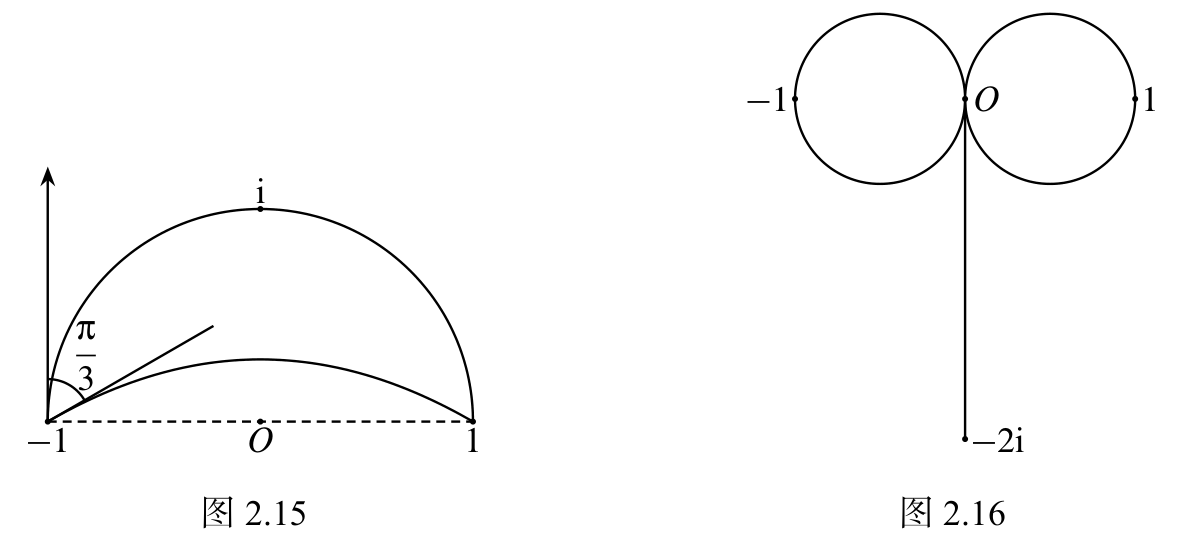
\includegraphics{public/figures/complex-functions/ch02-exercise-figures.png}
\caption{教材图 2.15 与图 2.16，分别对应习题 2.5 第 18、20 题}
\end{figure}

\par\Needspace{5\baselineskip}
\noindent\textbf{19.} 求一单叶全纯映射，把除去线段 \([1,2]\)
的单位圆盘的外部映为上半平面。

\par\Needspace{5\baselineskip}
\noindent\textbf{20.} 求一单叶全纯映射，把 \(B(-1/2;1/2)\) 和 \(B(1/2;1/2)\)
的外部除去线段 \([-2i,0]\) 所成的域（见图 2.16）映为上半平面。

校勘：第 19、20 题的外域按扩充平面包含 \(\infty\)
理解；否则一般会多一个穿孔，不能与上半平面双全纯等价。

\par\Needspace{5\baselineskip}
\noindent\textbf{21.} 设 \(0<r<a\)，求一单叶全纯映射，把域

\[
\{z\in\mathbb C:\operatorname{Re}z>0,\ |z-a|>r\}
\]

映为同心圆环

\[
\{w\in\mathbb C:\rho<|w|<1\}.
\]

\end{document}
